\documentclass[11pt,letterpaper]{article}
\usepackage[margin=0.88in,headheight=14pt]{geometry}
\usepackage[T1]{fontenc}
\usepackage[utf8]{inputenc}
\usepackage{lmodern,microtype}
\usepackage{amsmath,amssymb,bm}
\usepackage{booktabs,tabularx,array,longtable}
\usepackage{graphicx}
\usepackage[section]{placeins}
\usepackage[table]{xcolor}
\usepackage{siunitx}
\usepackage{listings,fancyhdr}
\usepackage{xurl}
\usepackage{hyperref}
\hypersetup{colorlinks=true,linkcolor=black,citecolor=black,urlcolor=blue!55!black,
  pdftitle={Reusable Launch Vehicle Simulator: Project 2},pdfauthor={Team 4}}
\sisetup{group-separator={,},group-minimum-digits=4,group-digits=integer}
\setlength{\emergencystretch}{2em}
\setlength{\tabcolsep}{5pt}
\renewcommand{\arraystretch}{1.18}
\newcolumntype{Y}{>{\raggedright\arraybackslash}X}
\newcommand{\code}[1]{\texttt{#1}}
\newcommand{\reportfigure}[3]{%
  \begin{figure}[!htbp]\centering
  \includegraphics[width=\textwidth,height=0.73\textheight,keepaspectratio]{report_assets/#1.pdf}
  \caption{#2}\label{#3}\end{figure}\FloatBarrier}
\makeatletter
\newcommand{\compactcontents}{%
  \begingroup\small
  \renewcommand{\l@section}[2]{\addvspace{2pt}%
    \@dottedtocline{1}{0pt}{1.5em}{\bfseries ##1}{\bfseries ##2}}%
  \tableofcontents\endgroup}
\makeatother
\lstset{basicstyle=\ttfamily\footnotesize,breaklines=true,columns=fullflexible,
  frame=single,rulecolor=\color{black!20},keepspaces=true,showstringspaces=false}
\pagestyle{fancy}\fancyhf{}
\lhead{RLV Simulator --- Project 2}\rhead{\thepage}
\setcounter{tocdepth}{2}

\begin{document}
\hypersetup{pageanchor=false}
\begin{titlepage}
\centering
\vspace*{1.5in}
{\LARGE\bfseries Reusable Launch Vehicle Simulator\par}
\vspace{0.2in}
{\Large Project 2 Report\par}
\vspace{0.5in}
{\large Guidance, Navigation, and Control System\par
for Reusable Launch Vehicles\par}
\vspace{0.15in}
{\large M2795.007800\par}
\vfill
{\large\textbf{Team 4}\par}
\vspace{0.15in}
{\large Anand \quad Jonas \quad Seongjae\par}
\vspace{0.35in}
{\large 10 November 2026\par}
\vfill
\end{titlepage}

\pagenumbering{roman}
\hypersetup{pageanchor=true}
\section*{Abstract}
\addcontentsline{toc}{section}{Abstract}
A modular six-degree-of-freedom simulation environment is developed for representative ascent and recovery phases of a Falcon~9 approximation. The model couples rigid-body motion, propellant-dependent mass properties, propulsion, aerodynamic loads, actuator response, and a rotating spherical Earth. Four prescribed-input experiments isolate ascent, entry burn, aerodynamic descent, and terminal powered descent; a fifth experiment evaluates closed-loop landing. Archived independent-reference comparisons give maximum position and velocity discrepancies of \SI{3.08e-6}{\metre} and \SI{4.23e-7}{\metre\per\second}. The landing case reaches contact at \SI{17.468}{\second} with approximately \SI{0.086}{\metre\per\second} speed and \SI{0.019}{\metre} position error under ideal actuation and truth-based state feedback. Comparison with CRS-11 webcast observations reveals substantial ascent mismatch, including an altitude RMSE of \SI{10.72}{\kilo\metre}; agreement with the implemented equations therefore does not establish flight fidelity. A separate synthetic IMU/GNSS/radar and 15-error-state ESKF study adds paired landing tests and fixed-truth replay. The navigation study includes uncertain initial alignment, missing-GNSS startup, multiple noise seeds, a 150-second ascent replay, and covariance-consistency diagnostics. Ten-seed soft-landing counts are 5/10 for the original landing configuration and 10/10 for the calibrated configuration; covariance diagnostics remain inconclusive. Sensor assumptions and the limits of these finite experiments are stated explicitly.
\clearpage
\compactcontents
\clearpage
\pagenumbering{arabic}

\section{Introduction}
\subsection{Project Objectives}
Project~2 requires a physics-based vehicle simulator and a navigation system for reusable launch vehicles. The simulator must predict how forces, moments, and propellant consumption change the vehicle state, and provide a basis for subsequent guidance and control design. Representative flight phases and public flight observations are used to assess the resulting motion. The navigation component must ultimately estimate position, velocity, attitude, and other required states from sensor measurements.

\subsection{Development Scope and Contributions}
The work presented here comprises the RLV-Sim vehicle model, its modular simulation interfaces, and five independently initialized flight experiments. The ascent model includes an attached upper assembly; recovery cases represent the booster alone. A prescribed-input mode separates the response of the physical model from feedback design. A closed-loop mode connects the same plant interface to a powered-descent planner, attitude controller, and actuator allocator.

The report evaluates the uncalibrated \code{project2\_*} scenario set. It documents the equations, experimental conditions, implementation checks, and agreement with CRS-11 altitude and speed observations. These independent cases do not constitute a continuous reconstructed mission. The numerical results use the archived verification campaign identified by the 3~November~2026 run IDs in Appendix~\ref{app:reproduction}; its stored trajectories have been reprocessed for the figures and flight-comparison statistics in this report. The navigation extension uses new 10~November executions of the original landing configuration and a separately identified calibrated landing configuration. The archived physics and public-flight comparison figures remain the uncalibrated baseline.

\subsection{Requirements and Evaluation Evidence}
The selected experiments address the Project~2 deliverables through the evidence below.
The prescribed phases and sensor-based navigation experiments have different acceptance
criteria; public-flight agreement is assessed separately from implementation correctness.
\begin{table}[!htbp]\centering\small
\caption{Project~2 requirements and evidence in this report.}\label{tab:requirements}
\begin{tabularx}{\textwidth}{lY}\toprule
Requirement & Evidence\\\midrule
Vehicle dynamics and reference frames & Coupled 6-DOF equations, variable mass properties,
rotating-Earth mechanics (Section~\ref{sec:models})\\
Environment and subsystems & Gravity, atmosphere, propulsion, aerodynamics, fins and
actuators (Section~\ref{sec:models})\\
Simulation architecture and code & Component interfaces, update timing and reproducible
commands (Section~\ref{sec:architecture}, Appendix~\ref{app:reproduction})\\
Sensor and navigation design & Native-force IMU, GNSS/radial height, initialization and
ESKF equations (Section~\ref{sec:navigation})\\
Representative phases and validation & Five independent cases, numerical verification
and CRS-11 observable comparison (Sections~\ref{sec:verification}--\ref{sec:results})\\
Navigation error analysis & Common-sample INS/ESKF comparison, multiple seeds,
initialization/outage studies and NEES/NIS (Section~\ref{sec:navigation-performance})\\
Engineering judgment and GNC risks & Parameter assumptions, model limits and consequences
for feedback design (Sections~\ref{sec:parameters}, \ref{sec:discussion})\\\bottomrule
\end{tabularx}
\end{table}
\FloatBarrier

\section{Simulation Architecture}\label{sec:architecture}
\subsection{System Components and Data Flow}
The implementation separates state definitions, plant construction, GNC components, and simulation execution. Table~\ref{tab:architecture} summarizes the responsibilities. Python resolves configurations and schedules module updates; a native C++ session advances the vehicle and actuator states.
\begin{table}[!htbp]
\centering\caption{Simulation components and exchanged information.}\label{tab:architecture}
\begin{tabularx}{\textwidth}{lYY}\toprule
Component & Responsibility & Principal information\\\midrule
Core & State definitions and frame conventions & Position, velocity, quaternion, angular rate, mass, timestamps\\
Plant & Forces, moments, mass properties, numerical propagation & Actuator inputs to vehicle truth and load diagnostics\\
GNC & Navigation, guidance, attitude control, allocation & State estimate to thrust and actuator commands\\
Simulation & Scheduling, logging, termination, evaluation & Time histories, contact metrics, resolved configuration\\\bottomrule
\end{tabularx}
\end{table}

For closed-loop operation, plant truth enters the navigation interface, which supplies an estimated state to guidance and control. Guidance requests a thrust vector; the attitude controller computes a body torque; the allocator converts these requests into throttle, gimbal, fin, and optional RCS commands. The plant holds each actuator command until the next scheduled update. In the baseline landing experiment, the navigation interface passes truth directly to the feedback laws. The navigation extension replaces this with a synthetic sensor generator and ESKF while retaining the plant and GNC settings within each paired test. The four prescribed-input cases instead apply a time-indexed command schedule without constructing GNC modules.

\subsection{Simulation Modes and Execution Timing}
The plant uses fixed-step fourth-order Runge--Kutta integration with quaternion normalization after each step. Navigation, guidance, control, and logging periods are integer multiples of the plant step. Timestamped outputs distinguish sampled states from interpolated surface-contact quantities. Separate native sessions and deterministic seeds allow repeatable episodes; each run stores its resolved configuration alongside the numerical histories. The periods used in this study are listed in Section~\ref{sec:settings}.

\subsection{Guidance and Control Used for the Landing Case}
The landing experiment uses an LCvx powered-descent planner, a per-axis PD attitude controller, and control allocation. Its 20-node convex planning problem imposes a \ang{15} thrust-pointing cone, a \ang{20} glideslope constraint, and hard terminal position and velocity conditions. The plan uses a local translational approximation and nominal gravity that includes the surface centrifugal contribution. A committed plan is tracked without repeated trajectory optimization. The plant continues to propagate the coupled rotating-Earth equations.

The outer tracking gains are $K_r=\operatorname{diag}(0.1,0.1,1.0)~\si{\per\second\squared}$ and $K_v=\operatorname{diag}(0.6,0.6,4.0)~\si{\per\second}$. Lower lateral gains account for the attitude response required to redirect thrust. These controllers provide a closed-loop test case; guidance optimization and controller design are not the principal subjects of this report.

\subsection{Visualization and Replay}\label{sec:replay}
The three-dimensional replay viewer reads the exported trajectory, attitude, configuration, and actuator histories. It displays vehicle motion together with flight telemetry, engine activity, gimbal and fin indicators, and RCS status. Timeline seeking, playback-speed controls, and selectable camera views support inspection of transitions and actuator response. Figure~\ref{fig:replay-landing} shows the interface during a landing demonstration; Appendix~\ref{app:replay} presents the other four flight phases.

The screenshots illustrate the interface using separate demonstration runs. Their displayed states and durations differ from the archived campaign analyzed in Section~\ref{sec:results}. The ocean and drone-ship scene supplies visual context, while the plant's radial-altitude calculation determines contact.
\begin{figure}[!htbp]
\centering
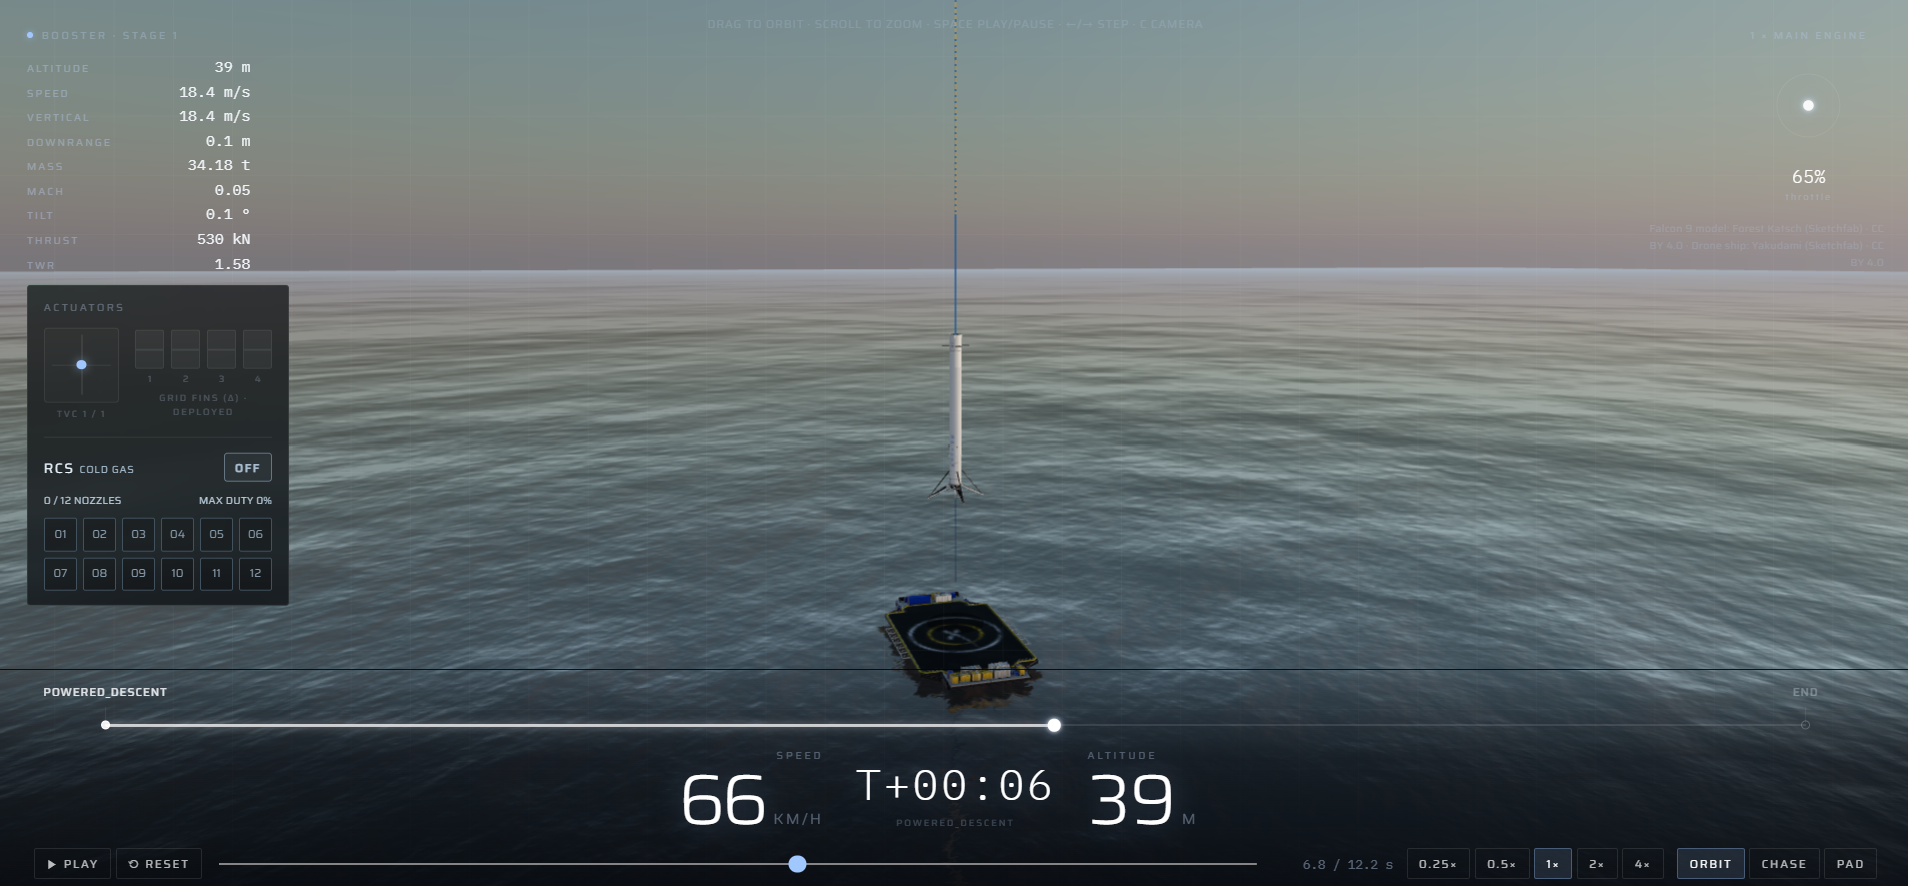
\includegraphics[width=\textwidth]{images/simulator_landing.png}
\caption{Replay interface during final approach. The central view shows vehicle attitude and deployed landing legs; the left and right panels display flight and actuator states, and the lower timeline provides replay controls. Vehicle model: Forest Katsch; drone ship: Yakudami (Sketchfab, CC BY 4.0).}
\label{fig:replay-landing}
\end{figure}
\FloatBarrier

\section{Vehicle and Environment Models}\label{sec:models}
\subsection{Reference Frames and State Definition}
The reference frame $N$ consists of Earth-fixed Cartesian axes aligned with North--East--Down at a selected spherical-surface origin. The axes remain fixed to Earth as the vehicle moves. The body frame $B$ has $+x$ toward the nose, $+y$ to the right, and $+z$ downward when level. Its geometric origin is at the nose, so engine and tank axial positions are negative. The scalar-first Hamilton quaternion $q_{BN}$ defines the rotation matrix $C_{BN}$ from body to reference components.

The rigid-body and propellant states are
\begin{equation}
\bm{x}=\left[\bm r^T,\bm v^T,q_{BN}^T,\bm\omega^T,m,m_g\right]^T,
\end{equation}
where $\bm r$ and $\bm v$ are Earth-relative position displacement and velocity, $\bm\omega$ is body angular velocity relative to the Earth-fixed axes, $m$ is total mass, and $m_g$ is RCS gas mass. Actuator internal states are propagated separately. For Earth radius $R_E$ and assumed origin latitude $\phi$,
\begin{equation}
\bm R_f=\bm r+[0,0,-R_E]^T,\qquad
h=\|\bm R_f\|-R_E,\qquad
\bm\Omega=\Omega_E[\cos\phi,0,-\sin\phi]^T.
\end{equation}
All three vectors are expressed in the fixed reference axes. Local downward direction is $\bm d_N=-\bm R_f/\|\bm R_f\|$. Radial altitude and vertical velocity are therefore distinct from $-r_D$ and $v_D$ far from the origin. Flight-path angle is defined by $\gamma=\sin^{-1}(-\bm v\cdot\bm d_N/\|\bm v\|)$, with positive values during climb. It is undefined at rest. Plots use body-axis tilt relative to radial upward direction to avoid the Euler-angle singularity at a vertical initial attitude.

\subsection{Translational and Rotational Equations of Motion}
For non-gravitational resultant body force $\bm F_b$, the free-flight equations are
\begin{align}
\dot{\bm r}&=\bm v,\\
\dot{\bm v}&=\frac{C_{BN}\bm F_b}{m}
-\frac{\mu\bm R_f}{\|\bm R_f\|^3}
-2\bm\Omega\times\bm v
-\bm\Omega\times(\bm\Omega\times\bm R_f).\label{eq:translation}
\end{align}
The terms represent applied force, central gravity, Coriolis acceleration, and centrifugal acceleration. A pad-reaction model holds the ascent vehicle before release. Surface contact is detected from radial altitude.

Rotational momentum balance uses the inertial angular velocity expressed in body axes,
\begin{equation}
\bm\omega_i=\bm\omega+C_{BN}^{T}\bm\Omega.
\end{equation}
With inertia tensor $I$ and resultant moment $\bm M_{CG}$ about the instantaneous CG, the implemented equations for the selected no-slosh cases are
\begin{align}
\dot q_{BN}&=\tfrac12 q_{BN}\otimes[0,\bm\omega]^T,\\
\dot{\bm\omega}&=I^{-1}\!\left[\bm M_{CG}
-\bm\omega_i\times(I\bm\omega_i)-\dot I\bm\omega_i\right]
+\bm\omega\times(C_{BN}^{T}\bm\Omega).\label{eq:rotation}
\end{align}
The moment includes engine, aerodynamic, grid-fin, and RCS contributions, together with the implemented exhaust angular-momentum flux. The latter is modeled as
\begin{equation}
\bm M_{jet}=-\beta_p(x_e-x_{CG})^2[0,\omega_{i,y},\omega_{i,z}]^T,
\end{equation}
where $\beta_p\geq0$ is main-propellant consumption rate. Using $\bm\omega_i$ in the angular momentum balance and $\bm\omega$ in quaternion propagation preserves the distinction between inertial and Earth-relative rates.

\subsection{Vehicle Configuration and Mass Properties}
Total mass is the sum of dry structure, any attached upper assembly, main propellant, and RCS gas. The main propellant occupies two cylindrical LOX/RP-1 tanks with fixed oxidizer-to-fuel mass ratio. Fill height determines each liquid component's CG and inertia. The combined properties follow
\begin{align}
\bm r_{CG}&=\frac{\sum_j m_j\bm r_j}{\sum_jm_j},\\
I&=\sum_j\left[I_{j,c}+m_j\left((\bm d_j^T\bm d_j)\mathbb I-\bm d_j\bm d_j^T\right)\right],
\quad \bm d_j=\bm r_j-\bm r_{CG},\\
\dot m&=-\beta_p-\beta_g,\qquad \dot m_g=-\beta_g.
\end{align}
Here $I_{j,c}$ is the component inertia about its own CG and $\beta_g$ is gas consumption rate. The inertia-rate contribution in Eq.~\eqref{eq:rotation} is evaluated as mass properties change.

The ascent configuration has an effective length of \SI{70}{\metre} and a \SI{120000}{\kilogram} attached upper assembly. Recovery configurations have a \SI{42}{\metre} body and no attached upper assembly. No separation event connects these experiments. The landing regression uses a distinct single-engine vehicle parameter set, summarized in Table~\ref{tab:hardware}; consequently its fuel margin cannot be appended to the recovery experiments as a continuous mission budget.

\subsection{Propulsion and Actuator Models}
For engine $i$, effective throttle $u_i$, vacuum thrust $T_{vac,i}$, ambient pressure $p_a$, and nozzle exit area $A_{e,i}$,
\begin{equation}
T_i=\max(u_iT_{vac,i}-p_aA_{e,i},0),\qquad
\beta_p=\sum_i\frac{u_iT_{vac,i}}{I_{sp,i}g_0}.
\end{equation}
Pressure reduces net thrust while mass flow is determined from the vacuum quantities. A gimballed engine produces $\bm F_i=T_i\hat{\bm d}_i$ and $\bm M_i=(\bm r_i-\bm r_{CG})\times\bm F_i$. Fuel availability limits both consumption and delivered impulse; depleted main propellant does not remove the separate RCS reserve.

The realistic actuator model uses a rate-limited throttle lag and a damped angular servo:
\begin{align}
\dot u&=r_u\tanh\!\left(\frac{u_c-u}{\tau r_u}\right),\\
\dot\delta&=v_\delta,\qquad
\dot v_\delta=2\zeta\omega_n\left[r_\delta\tanh\!\left(
\frac{\omega_n(\delta_c-\delta)}{2\zeta r_\delta}\right)-v_\delta\right].
\end{align}
Commands are clipped to throttle and deflection bounds; the minimum commanded nonzero throttle is 0.4. The prescribed-input runs use this actuator model, whereas landing uses ideal tracking of clipped commands. RCS capability includes 12 cold-gas nozzles, pulse-width modulation, and gas bookkeeping. RCS commands are zero in the reported experiments, so these phase results do not exercise RCS control authority.

\subsection{Aerodynamic and Grid-Fin Models}
The atmosphere co-rotates with Earth. For Earth-relative wind $\bm w_N$,
\begin{equation}
\bm v_a=C_{BN}^{T}(\bm v-\bm w_N),\quad V=\|\bm v_a\|,\quad
\bar q=\tfrac12\rho V^2,\quad M=V/a.
\end{equation}
The body model evaluates drag and lift coefficients from an analytically generated table, then assembles
\begin{align}
\bm F_a&=\bar qS(-C_D\hat{\bm v}_a+C_L\hat{\bm e}_L),\\
\bm M_a&=(x_{CP}-x_{CG})\bm e_x\times\bm F_a
-\frac{\bar qSL^2}{4V}[0,\omega_y,\omega_z]^T.
\end{align}
The lift direction $\hat{\bm e}_L$ is perpendicular to the flow, and zero-speed loads are set to zero. The table parameterization prescribes base drag, transonic and hypersonic changes, incidence dependence, and center-of-pressure movement. It is an engineering model, not a measured Falcon~9 aerodynamic database.

Ascent uses a nose-first table spanning Mach 0--12 and incidence \ang{0}--\ang{180}; recovery and landing use a base-first table spanning Mach 0--8 and incidence \ang{0}--\ang{90}. The reported angle of attack is relative to the selected aerodynamic forward axis ($+x$ in ascent and $-x$ in recovery), rather than always relative to the nose. This explains why a retrograde recovery attitude can have a small aerodynamic incidence.

For fin $j$, local flow includes body rotation, $\bm v_j=\bm v_a+\bm\omega\times(\bm r_j-\bm r_{CG})$. Lift and drag depend on fin incidence and local dynamic pressure; the fin moment is the mounting-arm cross product with its force. Each of four fins has nominal area \SI{2}{\square\metre}, with a smooth stall model based on a \ang{25} incidence scale. Deployment multiplies the aerodynamic loads by an exposure factor. Deployment motion, hinge impulse, stowed-fin drag, and structural flexibility are omitted.

\subsection{Gravity and Atmospheric Models}
All five cases use central gravity with $\mu=\SI{3.986004418e14}{\metre\cubed\per\second\squared}$, $R_E=\SI{6371000}{\metre}$, and $\Omega_E=\SI{7.292115e-5}{\radian\per\second}$. The reference latitude is assumed to be \ang{28.6} at each independently chosen origin. This is a spherical geocentric latitude, not a reconstructed geographic path.

The \code{ussa\_poly} atmosphere computes pressure and temperature from layered relations based on the U.S. Standard Atmosphere, 1976~\cite{ussa}. For geopotential altitude $h_g$, each layer has temperature $T=T_b+\lambda(h_g-h_b)$ and hydrostatic pressure relation $dp/dh_g=-g_0p/(R_aT)$. Density and sound speed follow $\rho=p/(R_aT)$ and $a=\sqrt{\gamma_aR_aT}$. The selected cases have no wind, temperature offset, or density dispersion. The ascent extends above the implementation's layer-boundary verification range of approximately \SI{84.85}{\kilo\metre}; its high-altitude continuation is an additional approximation, especially for the reported Mach number. This implementation limit is distinct from the wider altitude coverage of the published standard.

\subsection{Model Parameters and Their Sources}\label{sec:parameters}
Table~\ref{tab:hardware} lists the principal configured values. All vehicle-specific values in this table are modeling assumptions. Their numerical precision specifies the computation and does not indicate measurement accuracy.
\begin{table}[!htbp]
\centering\small
\caption{Principal hardware assumptions in the archived resolved configurations.}\label{tab:hardware}
\begin{tabularx}{\textwidth}{Yrrr}\toprule
Parameter & Ascent & Recovery cases & Landing\\\midrule
Dry structure [kg] & 25,000 & 25,000 & 25,600\\
Attached upper assembly [kg] & 120,000 & 0 & 0\\
Body length [m] & 70 & 42 & 42\\
Reference area [m$^2$] & 10.52 & 10.52 & 10.52\\
Vacuum thrust per engine [kN] & 914 & 914 & 981\\
Specific impulse [s] & 311 & 311 & 311\\
Nozzle exit area [m$^2$] & 0.68 & 0.68 & 0.90\\
Tank radius, LOX/RP-1 [m] & 1.8/1.8 & 1.8/1.8 & 1.7/1.7\\
Tank length, LOX/RP-1 [m] & 25/14 & 25/14 & 13/9\\
Liquid density, LOX/RP-1 [kg/m$^3$] & 1230/810 & 1230/810 & 1141/810\\
Initial RCS gas [kg] & 200 & 200 & 200\\\bottomrule
\end{tabularx}
\end{table}

The evidence categories are distinguished as follows. \emph{Published information} includes the course requirements and the public provenance of the CRS-11 data. \emph{Estimated quantities} include webcast-derived altitude/speed scales and any velocity components inferred during scenario preparation. \emph{Assumptions} include the remaining initial states, vehicle geometry and mass properties, propulsion values, aerodynamic coefficients, and prescribed commands. The versioned source and resolved configuration identify what was implemented; they are not independent evidence that a vehicle parameter is physically correct. The raw flight observations and their derived channels are distinguished in Section~\ref{sec:flightdata}.

\section{Navigation System}\label{sec:navigation}
% Shared navigation model for report.tex and main.tex.
\subsection{Navigation Architecture and Initialization}\label{sec:nav-architecture}
The synthetic IMU/GNSS/altimeter generator receives the native plant state and load
outputs. The 15-error-state ESKF receives only the resulting sensor samples, declared
reference-frame constants, and an uncertain initial alignment. Guidance and control use
its estimated state. Truth is retained separately for evaluation. The implementation is
\path{src/gnc/navigation/synthetic_eskf.py}, selected by
\path{gnc/navigation=synthetic_eskf}; \texttt{IdentityNav} supplies the ideal-feedback
comparison. The nominal and error states are
\begin{align}
 x_n&=(\bm r,\bm v,q_{BN},\bm b_g,\bm b_a),\\
 \delta\bm x&=[\delta\bm r^T,\delta\bm v^T,\delta\bm\theta^T,
                  \delta\bm b_g^T,\delta\bm b_a^T]^T.
\end{align}
Position and velocity use the same fixed-origin Cartesian reference axes as the plant.
Attitude error is expressed in reference axes, with a left multiplicative quaternion
correction. Mass is an ideal auxiliary measurement and is not estimated by this filter.

At startup, a synthetic preflight or handoff alignment observation is generated once:
\begin{equation}
 q_{align}=\operatorname{Exp}_q(\bm\epsilon_\theta)\otimes q_{true,0},
 \qquad\bm\epsilon_\theta\sim\mathcal N(0,\sigma_{align}^2 I),\quad
 \sigma_{align}=\ang{1}.
\end{equation}
This models an external coarse-alignment result with unknown error; it is not exact
attitude feedback or an autonomous cold-start alignment algorithm. No subsequent truth
quaternion is supplied to the estimator. Initial biases are zero, with standard
deviations of 0.05 deg/s and 0.1 m/s$^2$ for gyro and accelerometer bias.

When GNSS is available, its first position and velocity samples initialize the corresponding
state and covariance with the sensor variances; the same sample is not fused a second
time. Otherwise, an explicit launch-site or handoff position/velocity prior is used,
with 25 m and 2 m/s standard deviations per axis. This prior comes from the configured
nominal initial condition, independently of realized truth or dispersions. The outage
experiments deliberately perturb it. GNSS is fused normally when it becomes available.
Initialization without either GNSS or a declared prior is rejected before feedback begins.

\subsection{Physical Sensor Measurements}\label{sec:nav-sensors}
The IMU is modeled at the instantaneous vehicle CG. Native non-gravitational force and
inertial angular velocity generate its physical channels:
\begin{align}
 \widetilde{\bm f}_k&=\frac{\bm F_{non-grav,B,k}+\bm F_{pad,B,k}}{m_k}
                         +\bm b_a+\bm n_{a,k},\\
 \widetilde{\bm\omega}_{i,k}&=\bm\omega_{body,k}
                       +C(q_k)^T\bm\Omega+\bm b_g+\bm n_{g,k}.
\end{align}
Here $C(q)$ rotates body components into reference axes. Specific force includes pad
support and excludes gravitation: an ideal accelerometer reads zero in vacuum free fall
and a nonzero support acceleration on the pad. The gyro measures inertial body rate,
including Earth rotation even when the vehicle is stationary relative to Earth. These
channels are sampled directly from native force/rate diagnostics, without differentiating
truth velocity or using the filter's gravity model to generate the accelerometer signal.

GNSS measures reference-frame position and velocity; the altimeter measures radial height
above the modeled sphere:
\begin{align}
 \bm z_p&=\bm r+\bm n_p,&\bm z_v&=\bm v+\bm n_v,\\
 z_h&=\|\bm r+[0,0,-R_E]^T\|-R_E+n_h.
\end{align}
The altimeter is available from 0 to 1500 m height. In fixed-Earth experiments it instead
uses the plant's flat height $-r_D$. It is an ideal radial-height sensor, rather than a
model of a tilted radar beam and terrain intersection.

\begin{table}[!htbp]\centering\small
\caption{Assumed sensor parameters. White-noise levels are per-sample standard deviations,
per axis where applicable.}\label{tab:nav-sensors}
\begin{tabularx}{\textwidth}{lYY}\toprule
Channel & Rate / noise & Bias or availability\\\midrule
Accelerometer & 100 Hz; 0.08 m/s$^2$ & $(0.025,-0.020,0.035)$ m/s$^2$\\
Gyroscope & 100 Hz; 0.025 deg/s & $(0.005,-0.006,0.004)$ deg/s\\
GNSS position / velocity & 10 Hz; 2.5 m / 0.15 m/s & 3\% random loss per scheduled sample\\
Radial altimeter & 20 Hz; 0.5 m & 0--1500 m height\\
Initial alignment & Once; 1 deg & Independent reference-axis rotation error\\\bottomrule
\end{tabularx}
\end{table}
Noise streams are deterministic functions of episode seed, epoch, and channel. The
injected IMU biases are constant; the filter permits bias adaptation through process
noise. Sensor noise, bias, and alignment values are engineering assumptions, not
identified Falcon~9 hardware specifications. Optional scale factors, bias random walks,
GNSS gross-error injection, and innovation gates are available for separate mismatch
experiments; they are disabled in the nominal campaign. GNSS interruption is selected
only in the explicitly labeled outage trials. Sensor latency, misalignment, saturation,
lever arms, vibration, and quantization are outside this model. Standalone
post-processed sensor CSVs are not the samples fused by this online ESKF.

\subsection{Rotating-Frame INS and ESKF}\label{sec:nav-filter}
For $\bm R=\bm r+[0,0,-R_E]^T$, bias-corrected measurements
$\bm f=\widetilde{\bm f}-\widehat{\bm b}_a$ and
$\bm\omega_i=\widetilde{\bm\omega}_i-\widehat{\bm b}_g$, the mechanization is
\begin{align}
 \dot{\widehat{\bm r}}&=\widehat{\bm v},\\
 \dot{\widehat{\bm v}}&=C(\widehat q)\bm f
   -\frac{\mu\widehat{\bm R}}{\|\widehat{\bm R}\|^3}
   -2\bm\Omega\times\widehat{\bm v}
   -\bm\Omega\times(\bm\Omega\times\widehat{\bm R}),\\
 \widehat q_k^-&=\operatorname{Exp}_q(-\bm\Omega\Delta t)\otimes
   \widehat q_{k-1}^+\otimes\operatorname{Exp}_q(\overline{\bm\omega}_i\Delta t).
\end{align}
Neighboring IMU samples are averaged, and the midpoint attitude rotates the specific
force. Translation uses RK4 over each navigation interval with that held midpoint force.
The frame acceleration is evaluated at the RK stages. This is a sampled mechanization;
subsample coning, sculling, and actuator discontinuities are not resolved by averaging.
The fixed-Earth mode uses its configured vertical gravity law and zero Earth rotation.
The rate returned to control is
$\widehat{\bm\omega}_{body}=\widetilde{\bm\omega}_i-\widehat{\bm b}_g
-C(\widehat q)^T\bm\Omega$.

Let $W=[\bm\Omega]_\times$, $A=C\bm f$, and
$J_g=\mu(3\bm R\bm R^T/\|\bm R\|^5-I/\|\bm R\|^3)$. The reference-frame
error linearization, using the global angular-error convention~\cite{sola}, is
\begin{equation}
 F=\begin{bmatrix}
 0&I&0&0&0\\
 J_g-W^2&-2W&-[A]_\times&0&-C\\
 0&0&-W&-C&0\\
 0&0&0&0&0\\
 0&0&0&0&0
 \end{bmatrix},\qquad
 \Phi=I+F\Delta t+\tfrac12F^2\Delta t^2.
\end{equation}
The fixed-mode gravity Jacobian replaces $J_g$ where applicable. Covariance propagation is
$P^- =\Phi P^+\Phi^T+BDB^T$, where $B=(I+\tfrac12F\Delta t)G$ and $G$ maps
accelerometer noise into velocity through $C$, gyro noise into attitude through $C$, and
bias noise into the two bias blocks. The noise variances in $D$ are
$\sigma_a^2\Delta t^2$, $\sigma_g^2\Delta t^2$, $s_{bg}^2\Delta t$, and
$s_{ba}^2\Delta t$, each repeated three times. The assumed bias-process amplitudes are
$s_{bg}=0.0005$ deg/s$/\sqrt{\mathrm{s}}$ and
$s_{ba}=0.0005$ m/s$^2/\sqrt{\mathrm{s}}$. This discrete noise approximation does not
explicitly augment the correlated noise introduced by neighboring-sample averaging;
its covariance behavior is evaluated empirically in the consistency study.

For innovation $\bm y=\bm z-h(\widehat x^-)$,
\begin{align}
 S&=HP^-H^T+R,&K&=P^-H^TS^{-1},&\delta\widehat{\bm x}&=K\bm y,\\
 P_J&=(I-KH)P^-(I-KH)^T+KRK^T.
\end{align}
GNSS selects position and velocity. The radial-height Jacobian is
$H_{h,r}=\widehat{\bm R}^T/\|\widehat{\bm R}\|$.
Optional innovation gates reject an update when $\bm y^TS^{-1}\bm y$ exceeds a
configured threshold; the nominal results use ungated valid measurements.
Position, velocity, and bias corrections are additive; attitude is corrected on the left,
$\widehat q^+=\operatorname{Exp}_q(\delta\widehat{\bm\theta})\otimes\widehat q^-$.
After injection, covariance is reset as $P^+=G_rP_JG_r^T$, where the attitude block of
$G_r$ is the SO(3) left Jacobian
\begin{equation}
 J_l(\bm\phi)=I+\frac{1-\cos\theta}{\theta^2}[\bm\phi]_\times
 +\frac{\theta-\sin\theta}{\theta^3}[\bm\phi]_\times^2,
 \qquad\theta=\|\bm\phi\|,
\end{equation}
with its small-angle limit near zero. Covariance is symmetrized after propagation and
correction. Innovation statistics and the full-state estimation error are evaluated
separately from quaternion normalization and covariance positivity.


\section{Simulation Cases and Experimental Setup}\label{sec:experiments}
\subsection{Case Selection and Evaluation Objectives}
The five cases cover different dominant mechanisms. Ascent tests thrust, pitch excitation, aerodynamic loading, and a large change in mass. Entry burn tests three-engine deceleration and shutdown. Aerodynamic descent isolates unpowered atmospheric loads. Terminal powered descent tests single-engine braking and shutdown while still airborne. Landing evaluates feedback-driven contact. Each case starts from its own initial condition; states and propellant are not transferred between cases.

\subsection{Initial Conditions and Prescribed Inputs}
Table~\ref{tab:initial} gives the initial states; all cases begin with zero body angular rate, zero roll, and \SI{200}{\kilogram} RCS gas. Horizontal position is zero at the chosen origin. The recovery heading is synthetic. The initial recovery attitude aligns the thrust axis against the initial velocity, but attitude subsequently evolves under the full rotational equations.
\begin{table}[!htbp]
\centering\small
\caption{Initial conditions. Velocity components use the fixed NED axes; angles use intrinsic ZYX Euler initialization.}\label{tab:initial}
\begin{tabularx}{\textwidth}{Yrrrrr}\toprule
Case & $h$ [m] & $(v_N,v_E,v_D)$ [m/s] & $m$ [kg] & Pitch [$^\circ$] & Yaw [$^\circ$]\\\midrule
Ascent & 0 & $(0,0,0)$ & 545,200 & 90.000 & 45\\
Entry burn & 47,500 & $(406.914,0,1192.778)$ & 40,000 & 71.163 & 180\\
Aero descent & 35,000 & $(480.561,0,823.992)$ & 34,000 & 59.749 & 180\\
Powered descent & 4,700 & $(142.691,0,286.067)$ & 32,000 & 63.490 & 180\\
Landing & 300 & $(0,0,25)$ & 29,500 & 90.000 & 0\\\bottomrule
\end{tabularx}
\end{table}

In ascent, nine engines start at full throttle with the vehicle on the pad. A \SI{0.002}{\radian} pitch-gimbal command acts from 10 to \SI{12}{\second}. Throttle is reduced to 0.8 from 50 to \SI{74}{\second}, restored to 1, and commanded off at \SI{145}{\second}. Propagation continues to \SI{150}{\second}. Fins remain stowed. The schedule is prescribed rather than derived from a flight-guidance law.

Entry burn activates engines 0, 1, and 5 at throttle 0.50, commands cutoff at \SI{12}{\second}, and ends at \SI{14}{\second}. Aerodynamic descent keeps the engines off for \SI{45}{\second}. Powered descent uses the center engine at throttle 0.55 for \SI{20}{\second}, followed by \SI{2}{\second} shutdown observation. These three cases start with zero actual throttle and expose neutral fins throughout; gimbal, fin-deflection, and RCS commands remain zero.

\subsection{Closed-Loop Landing Configuration}
Landing begins at \SI{300}{\metre} with \SI{25}{\metre\per\second} downward speed and \SI{3700}{\kilogram} main propellant. The target is the surface origin. The single-engine model in Table~\ref{tab:hardware}, ideal actuation, and truth feedback isolate nominal closed-loop behavior. RCS allocation and initial-state dispersions are disabled. The episode ends at surface contact or a \SI{40}{\second} horizon.

\subsection{Numerical Settings and Evaluation Criteria}\label{sec:settings}
The nominal plant step is \SI{1}{\milli\second}. Prescribed commands update every \SI{20}{\milli\second}; logging uses \SI{200}{\milli\second} in ascent and \SI{20}{\milli\second} in the other prescribed cases. Landing uses navigation, control, guidance, and logging periods of 10, 20, 1000, and \SI{100}{\milli\second}, respectively, with zero command-delay ticks. A guidance update does not imply a new trajectory optimization when replanning is disabled.

For prescribed experiments, evaluation includes finite states, mass and gas bookkeeping, quaternion norm, shutdown behavior, aerodynamic-table coverage, independent-reference error, and step-size agreement. The landing configuration bounds position error by \SI{10}{\metre}, total speed by \SI{5}{\metre\per\second}, and tilt by \ang{15}. Success additionally requires the runner's tighter soft-contact classification: downward speed at most \SI{2}{\metre\per\second}, lateral speed at most \SI{1}{\metre\per\second}, tilt at most \ang{5}, and angular-rate magnitude at most \SI{0.1}{\radian\per\second}, with positive remaining propellant. These are configured experimental criteria; they are not flight qualification limits. Comparison with public observations uses continuous residuals rather than a pass/fail threshold.

\section{Model and Numerical Verification}\label{sec:verification}
\subsection{Verification Methods and Reference Solutions}
The verification campaign combines component checks with independently integrated full-phase equations. For the four prescribed cases, a configuration-based DOP853 implementation calculates forces, mass properties, and motion without calling the production force or frame routines. Reference attitude is propagated as a rotation matrix. Rotating-Earth reference trajectories are integrated in inertial coordinates and transformed back to the stored frame, reducing the risk of reproducing the same rotating-frame implementation error.

The maximum sampled vector error is $e_{x,\max}=\max_k\|\bm x_{sim}(t_k)-\bm x_{ref}(t_k)\|_2$. Attitude error is the principal relative rotation angle. Table~\ref{tab:verification} reports the archived full-phase discrepancies. Separate canonical tests in the implementation record cover free fall, vacuum burn, torque-free rotation, propulsion, fin loads, and atmospheric layer boundaries. Their parameters need not equal those of the five phase experiments.
\begin{table}[!htbp]
\centering\small
\caption{Maximum native/reference differences for the selected archived phase runs.}\label{tab:verification}
\begin{tabular}{lrrrr}\toprule
Case & Position [m] & Velocity [m/s] & Attitude [rad] & Mass [kg]\\\midrule
Ascent & $3.08\times10^{-6}$ & $4.23\times10^{-7}$ & $1.51\times10^{-10}$ & $2.27\times10^{-5}$\\
Entry burn & $1.91\times10^{-6}$ & $2.19\times10^{-7}$ & $1.46\times10^{-11}$ & $2.52\times10^{-7}$\\
Aero descent & $2.41\times10^{-6}$ & $3.58\times10^{-7}$ & $2.44\times10^{-11}$ & 0\\
Powered descent & $3.17\times10^{-7}$ & $2.81\times10^{-8}$ & $2.06\times10^{-11}$ & $3.31\times10^{-7}$\\\midrule
Acceptance limit & $10^{-2}$ & $10^{-3}$ & $10^{-6}$ & $10^{-3}$\\\bottomrule
\end{tabular}
\end{table}

\subsection{Integration Accuracy and Step-Size Convergence}
Native runs at 2, 1, and \SI{0.5}{\milli\second} were compared at shared output times. Across the four prescribed cases and both adjacent step pairs, the largest position and velocity differences were \SI{2.08e-6}{\metre} and \SI{2.90e-7}{\metre\per\second}. The corresponding acceptance limits were \SI{0.1}{\metre} and \SI{0.01}{\metre\per\second}. The largest adjacent-step mass difference was \SI{4.17e-6}{\kilogram}, below the \SI{0.01}{\kilogram} limit.

These differences establish numerical agreement at the tested resolutions, but not a measured fourth-order convergence rate. For example, the ascent position difference increases between the finer pair. Very small errors, event handling, reference accuracy, and floating-point effects can obscure the asymptotic integration order. Reference tolerances were also tightened separately; in the selected entry-burn record, the resulting mass difference is \SI{3.04e-5}{\kilogram}.

\subsection{Physical Consistency and Subsystem Checks}
The archived phase records show zero mass-bookkeeping error, nonnegative propellant, no spurious mass increase, and quaternion-norm errors below $3\times10^{-16}$. Main-engine force is zero at the end of each prescribed experiment. RCS gas remains constant because no RCS activity is commanded. Maximum angles of attack in ascent, entry burn, aerodynamic descent, and powered descent are \ang{0.968}, \ang{0.808}, \ang{0.766}, and \ang{0.726}, respectively. Ascent reaches Mach 8.625 and therefore requires its Mach-12 table rather than the recovery table.

The separate rotating-Earth verification includes full-orbit and asymmetric torque-free problems. At a \SI{0.5}{\second} step, the recorded maximum orbital position error against a Kepler solution is \SI{1.08e-6}{\metre}; conservation checks cover inertial energy and angular momentum. These tests evaluate the central-gravity and frame implementation under smooth test conditions.

\subsection{Verification Results}
All five selected archived verification records are marked passed. The landing record checks contact, the configured success criteria, and physical bookkeeping; it does not use the prescribed-input DOP853 comparison. Thus the landing success and the independent-equation errors in Table~\ref{tab:verification} are different forms of evidence.

The five representative phase checks were also reproduced with the submitted implementation. All passed their configured criteria. In entry burn, the reference mass-refinement difference was \SI{3.04e-5}{\kilogram}, below the \SI{1e-4}{\kilogram} stability limit. The numerical tolerances assess agreement with the declared equations, independently of the flight-data residuals.

\section{Simulation Results and Flight-Data Comparison}\label{sec:results}
Table~\ref{tab:results} summarizes the five cases. The prescribed cases report their final native sample; landing reports quantities interpolated to radial surface contact. Figures in this section are regenerated from the archived state and diagnostic histories.
\begin{table}[!htbp]
\centering\small
\caption{Final states and remaining main propellant.}\label{tab:results}
\begin{tabularx}{\textwidth}{Yrrrr}\toprule
Case & Time [s] & Altitude [km] & Speed [m/s] & Propellant [kg]\\\midrule
Ascent & 150 & 101.056 & 2171.271 & 20,654.7\\
Entry burn & 14 & 33.000 & 944.131 & 9576.2\\
Aero descent & 45 & 3.758 & 310.462 & 8800.0\\
Powered descent & 22 & 1.528 & 80.630 & 3557.7\\
Landing (contact) & 17.468 & 0 & 0.086 & 1378.8\\\bottomrule
\end{tabularx}
\end{table}

\subsection{Powered Ascent}
The ascent reaches \SI{101.056}{\kilo\metre} after \SI{150}{\second}, while main propellant decreases from 400,000 to approximately \SI{20655}{\kilogram}. Figure~\ref{fig:ascent} shows the imposed throttle reduction and subsequent return to full thrust. Net thrust also changes with ambient pressure. The large mass decrease increases the acceleration available from a given thrust, contributing to the steeper late-time speed rise.

Dynamic pressure peaks at \SI{31.01}{\kilo\pascal} near \SI{50.6}{\second}, shortly after the throttle-reduction command. The peak reflects the competing effects of increasing speed and decreasing atmospheric density, with actuator lag affecting the immediate thrust response. After cutoff at \SI{145}{\second}, propellant consumption stops as thrust decays; altitude continues to rise while speed decreases. At that command epoch, altitude and speed are \SI{91.620}{\kilo\metre} and \SI{2190.20}{\metre\per\second}.

The maximum aerodynamic incidence remains below \ang{1}; the body therefore remains approximately aligned with the velocity even as the path bends away from vertical. This is a response to the chosen pitch excitation and subsequent dynamics, not evidence that an operational pitch program has been recovered. Body-axis tilt and angular-rate histories are provided in Appendix~\ref{app:supplement}.
\reportfigure{ascent}{Powered ascent. The thrust reduction at 50--74 s, cutoff at 145 s, dynamic-pressure maximum, and declining propellant mass are shown on the same elapsed-time basis. Horizontal distance is measured from this experiment's origin.}{fig:ascent}

\subsection{Entry Burn and Aerodynamic Descent}
Entry burn reduces speed from \SI{1260.3}{\metre\per\second} to \SI{944.1}{\metre\per\second} over \SI{14}{\second}, consuming approximately \SI{5224}{\kilogram} of main propellant. Figure~\ref{fig:entry} shows thrust build-up from an initially unthrottled engine state and shutdown after the \SI{12}{\second} cutoff command. Despite decreasing speed, dynamic pressure reaches \SI{5.16}{\kilo\pascal} at the end of the interval: descent into denser air offsets the reduction in $V^2$.
\reportfigure{entry_burn}{Entry burn. Three engines brake the descending vehicle; the final two seconds expose the shutdown transient. Dynamic pressure increases as the vehicle enters denser atmosphere.}{fig:entry}

In aerodynamic descent, speed falls from \SI{953.9}{\metre\per\second} to \SI{310.5}{\metre\per\second} without thrust or propellant consumption. Body and neutral-fin aerodynamic loads supply the deceleration. The dynamic-pressure maximum is \SI{84.33}{\kilo\pascal} at \SI{29.18}{\second}; after this point, the speed reduction dominates the continuing density increase. This peak is a load prediction under the assumed coefficients and initial state, not a demonstrated structural margin.

The flight-path angle changes from approximately $-\ang{59.75}$ to $-\ang{73.80}$, while maximum incidence is \ang{0.766}. The vehicle ends at \SI{3.758}{\kilo\metre}, still descending. Neutral fin commands do not imply zero fin loads because both translational and rotational local flow enter the fin model.
\reportfigure{aero_descent}{Aerodynamic descent with engines off and exposed neutral fins. Constant propellant mass separates aerodynamic braking from powered deceleration; the load maximum occurs before the final low-speed portion.}{fig:aero}

\subsection{Terminal Powered Descent and Landing}
The prescribed powered-descent case reduces speed from \SI{319.7}{\metre\per\second} to \SI{80.6}{\metre\per\second}, leaving \SI{3557.7}{\kilogram} main propellant. Dynamic pressure is greatest initially, at \SI{38.86}{\kilo\pascal}, and decreases during braking. At \SI{22}{\second}, altitude is still \SI{1.528}{\kilo\metre}; the final radial downward speed is approximately \SI{80.41}{\metre\per\second}. This case demonstrates braking and shutdown response without imposing a touchdown boundary condition.
\reportfigure{powered_descent}{Prescribed terminal powered descent. The center engine is commanded off at 20 s; the run ends while the vehicle remains airborne.}{fig:powered}

The separate landing case starts at \SI{300}{\metre} and reaches contact at \SI{17.468}{\second}. Interpolated contact speed is \SI{0.086}{\metre\per\second}, position error is \SI{0.019}{\metre}, and tilt is \ang{0.055}. Approximately \SI{2321}{\kilogram} main propellant is consumed, leaving \SI{1378.8}{\kilogram}. The case satisfies its configured contact criteria.

The maximum dynamic pressure is only \SI{0.372}{\kilo\pascal}, making this chiefly a thrust-and-feedback experiment. Near contact, angle of attack increases as total speed becomes very small; this does not imply a comparable growth in aerodynamic force because dynamic pressure approaches zero. The terminal native sample occurs slightly below the surface, so its \SI{0.08456}{\metre\per\second} speed is distinct from the interpolated contact result. Contact detection does not model landing-leg impact dynamics.
\reportfigure{landing}{Closed-loop landing under ideal actuation and truth feedback. The time history ends at the first below-surface native sample; the reported touchdown metrics are interpolated to zero radial altitude.}{fig:landing}

\subsection{Comparison with CRS-11 Flight Data}\label{sec:comparison}
\subsubsection{Data Sources and Processing}\label{sec:flightdata}
The reference is the CRS-11 stage-1 raw data in the public \emph{Telemetry-Data} repository, pinned to commit \code{b245d3b81aa36b7941ec10f3f4b508999d106a6d}~\cite{telemetry}. The local manifest, \path{data/reference/crs11/manifest.json}, records source URLs, byte counts, and SHA-256 hashes. The approximately \SI{0.033}{\second} samples contain numbers extracted from the webcast time, altitude, and speed displays. They are not raw onboard sensor measurements. Altitude is converted from kilometres to metres; the stored velocity is in metres per second.

The reference dataset distinguishes raw displayed observables from analysed channels, including derived vertical velocity, downrange, and dynamic pressure~\cite{telemetry}. Only raw altitude and total speed are compared here. Display quantization, extraction errors, unknown processing delay, and uncertain altitude and speed reference conventions limit interpretation. The extraction cadence does not establish an independent sensor sampling rate or measurement accuracy.

\subsubsection{Comparison Conditions and Error Metrics}
Simulation elapsed time is mapped to mission time with fixed starts of 0, 372, 384, and \SI{429}{\second} for ascent, entry burn, aerodynamic descent, and powered descent. Requested reference windows end at 145, 384, 429, and \SI{462}{\second}. The powered-descent run covers only the first \SI{22}{\second} of its window. The independently initialized landing regression has no assigned flight-data comparison.

The comparison assumes equal altitude datums and Earth-relative speed, with zero altitude offset. Simulated observables are linearly interpolated at overlapping reference timestamps, and the exact initial simulation epoch is excluded. No extrapolation is used. For residual $e_k=y_{sim,k}-y_{obs,k}$, the time-weighted bias and RMSE are
\begin{align}
b&=\frac{1}{D}\sum_{k\in\mathcal K}\frac{e_k+e_{k+1}}{2}\Delta t_k,\\
\operatorname{RMSE}&=\left[\frac{1}{D}\sum_{k\in\mathcal K}
\frac{e_k^2+e_{k+1}^2}{2}\Delta t_k\right]^{1/2},
\quad D=\sum_{k\in\mathcal K}\Delta t_k.
\end{align}
Only intervals $0<\Delta t_k\leq\SI{1.1}{\second}$ belong to $\mathcal K$, preventing missing coverage from receiving interpolation weight. The duration in Table~\ref{tab:comparison} is this covered duration, which can be shorter than the timestamp span.

\subsubsection{Comparison Results and Error Analysis}
\begin{table}[!htbp]
\centering\small
\caption{Time-weighted comparison with CRS-11 raw altitude and speed. Positive bias means the simulation overpredicts the observable.}\label{tab:comparison}
\begin{tabularx}{\textwidth}{Yrrrrr}\toprule
Case & Coverage & Altitude bias & Altitude RMSE & Speed bias & Speed RMSE\\
 & [s] & [m] & [m] & [m/s] & [m/s]\\\midrule
Ascent & 143.643 & 7365.0 & 10721.6 & 160.8 & 203.0\\
Entry burn & 11.979 & $-103.3$ & 135.1 & $-11.4$ & 22.1\\
Aero descent & 44.979 & 250.1 & 650.0 & 43.3 & 59.9\\
Powered descent & 21.955 & 503.0 & 617.8 & $-53.6$ & 56.1\\\bottomrule
\end{tabularx}
\end{table}

Figure~\ref{fig:flight} shows that ascent increasingly overpredicts both altitude and speed. At the same mission epoch, \SI{145}{\second}, simulated altitude is \SI{91.620}{\kilo\metre}, compared with \SI{62.400}{\kilo\metre} obtained by interpolating the raw observations; simulated and observed speeds are \SI{2190.20}{\metre\per\second} and \SI{1684.44}{\metre\per\second}. The same-time discrepancies are therefore approximately \SI{29.22}{\kilo\metre} and \SI{505.76}{\metre\per\second}. Comparing the later \SI{150}{\second} simulation endpoint with MECO would confound this difference with additional coast time.

The systematic ascent mismatch indicates that the prescribed thrust history, mass budget, trajectory orientation, and assumed aerodynamic/environment models do not jointly reproduce the observed flight. Their separate contributions are not identified by this comparison. The increasing residual is much larger than the numerical integration discrepancies, so reducing the timestep alone will not address it. A controlled parameter study and better-constrained input history are needed before selecting a correction.

Entry burn has the smallest altitude RMSE, but its initial scale and burn window are selected from the flight context. Agreement over this short interval therefore provides limited evidence about prediction outside that window. In aerodynamic descent, a positive speed bias of \SI{43.3}{\metre\per\second} indicates underpredicted deceleration on average. Possible contributors include aerodynamic coefficients, initial velocity direction, and mass; a nearly matched terminal speed does not eliminate the intermediate mismatch. In powered descent, positive altitude bias together with negative speed bias is consistent with excessive braking and/or a different descent geometry. These are candidate explanations rather than established parameter diagnoses.

The comparison tests agreement in two observables. It neither identifies a unique six-degree-of-freedom trajectory nor measures navigation error. No model parameters were fitted in this baseline comparison. Residual histories are included in Appendix~\ref{app:supplement}.
\reportfigure{flight_comparison}{Simulated and webcast-derived altitude and speed on a common mission-time axis. Each row is an independently initialized experiment. Point markers preserve visible gaps in the observational record.}{fig:flight}

\section{Navigation Performance}\label{sec:navigation-performance}
% Shared by main.tex and report.tex; numerical tables are generated from executed runs.
\subsection{Experiment Design and Error Definitions}\label{sec:nav-experiments}

The navigation campaign was executed on 10 November 2026 using
\path{report_assets/generate_navigation.py}, with the physically sampled ESKF and
seed~0 for the paired comparisons, supplemented by the multi-seed experiments below. It supplements the earlier physics campaign. Two paired closed-loop tests use
\path{project2_landing} and \path{flight_calibrated_landing}. Within each pair,
the resolved configuration is identical except for the navigation module; the generation
script checks that invariant. Initial-state dispersion is disabled. Each run propagates
its own closed-loop trajectory, so the comparison measures the effect of navigation on
the combined estimation, planning, and control response.

The Project~2 pair starts at 300 m and 25 m/s downward speed, with ideal actuators and a
free-terminal-time LCvx plan. The calibrated pair starts at 348.764 m and 76.111 m/s
downward speed, with mass 35,692.161 kg, realistic actuators, and the scenario's previously
selected aerodynamic parameters. Its LCvx plan uses a 12.145 s terminal time, a 30 kN/s
planned thrust-rate limit, and vertical tracking gains of 6 s$^{-2}$ and 4 s$^{-1}$.
These settings originate from the separate flight-calibration study; no parameters are
refitted to the sensor samples. Neither differences between these two scenario families
nor the calibrated scenario's fit to public observables are treated as navigation errors.
Both use a 1 ms plant step, 10 ms navigation period, and 20 ms control period. The guidance
interface is called every second, but \texttt{convex\_replan=false} retains the initial plan
while tracking feedback continues. Trajectory logging periods remain 100 ms and 20 ms,
respectively; all navigation errors use the full 10 ms navigation grid.

For vector state $\bm x$, error magnitude and reported summary statistics are
\begin{equation}
 e_k=\|\widehat{\bm x}_k-\bm x_{truth,k}\|_2,\qquad
 \mathrm{RMSE}=\sqrt{\frac1N\sum_{k=1}^{N}e_k^2},\qquad e_{\max}=\max_k e_k.
\end{equation}
Attitude error is the shortest relative-quaternion rotation angle, reported in degrees;
angular-rate error is the norm of the body/reference rate difference, reported in degrees
per second. Initialization transients are included. Navigation samples stop at the last
scheduled update before the plant terminates. Ground-contact speed, miss distance, and
tilt use the simulator's interpolation to zero radial altitude; contact time in the tables
is interpolated with the same logged-state bracket. These terminal quantities and the
navigation samples are therefore evaluated at distinct epochs.

\subsection{Closed-Loop Navigation and Landing Results}\label{sec:nav-closed-loop}

All four nominal cases reach a soft landing under the existing simulator criteria.
Table~\ref{tab:nav-contact} compares the paired terminal results and
Table~\ref{tab:nav-errors} reports ESKF accuracy against each run's own truth.
Identity navigation has exactly zero estimation error because it returns truth.
It is an ideal-feedback reference, not an unfiltered sensor estimator.

\begin{table}[!htbp]\centering\small
\caption{Paired closed-loop results, seed 0. Each pair changes only navigation.
All four cases satisfy the simulator's soft-landing and success criteria.}\label{tab:nav-contact}
% Generated by report_assets/generate_navigation.py; do not edit numbers.
\begin{tabularx}{\textwidth}{ll*{4}{>{\raggedleft\arraybackslash}X}}\toprule
Scenario & Navigation & Contact [s] & Speed [m/s] & Miss [m] & Tilt [deg]\\\midrule
Project 2 & Identity & 17.468 & 0.086 & 0.019 & 0.055\\
Project 2 & ESKF & 17.583 & 1.381 & 0.788 & 0.219\\
Calibrated & Identity & 12.230 & 0.483 & 0.014 & 0.062\\
Calibrated & ESKF & 12.195 & 0.553 & 0.602 & 1.097\\
\bottomrule\end{tabularx}

\end{table}

\begin{table}[!htbp]\centering\small
\caption{ESKF navigation error statistics on the full navigation grid. Vector entries use
norms, not componentwise averages.}\label{tab:nav-errors}
\begin{tabularx}{\textwidth}{ll*{4}{>{\raggedleft\arraybackslash}X}}\toprule
Scenario & Statistic & Position [m] & Velocity [m/s] & Attitude [deg] & Rate [deg/s]\\\midrule
Project 2 & RMSE & 0.540 & 0.066 & 1.356 & 0.048\\
Project 2 & MAX & 2.879 & 0.182 & 2.444 & 0.131\\
Calibrated & RMSE & 0.641 & 0.074 & 1.189 & 0.049\\
Calibrated & MAX & 2.879 & 0.166 & 2.282 & 0.125\\
\bottomrule\end{tabularx}

\end{table}
\FloatBarrier

The ESKF introduces observable feedback consequences. In the Project~2 pair, contact speed
increases from 0.086 to 1.381 m/s while the position-estimation RMSE is 0.540 m. In the
calibrated pair, contact speed changes from 0.483 to 0.553 m/s and horizontal miss increases
from 0.014 to 0.602 m, with position-estimation RMSE 0.641 m. Thus sub-metre average
estimation error does not imply unchanged terminal performance. The plots show estimation
transients and the resulting trajectories; they do not establish robustness probabilities
from a single noise realization.

\begin{figure}[!htbp]\centering
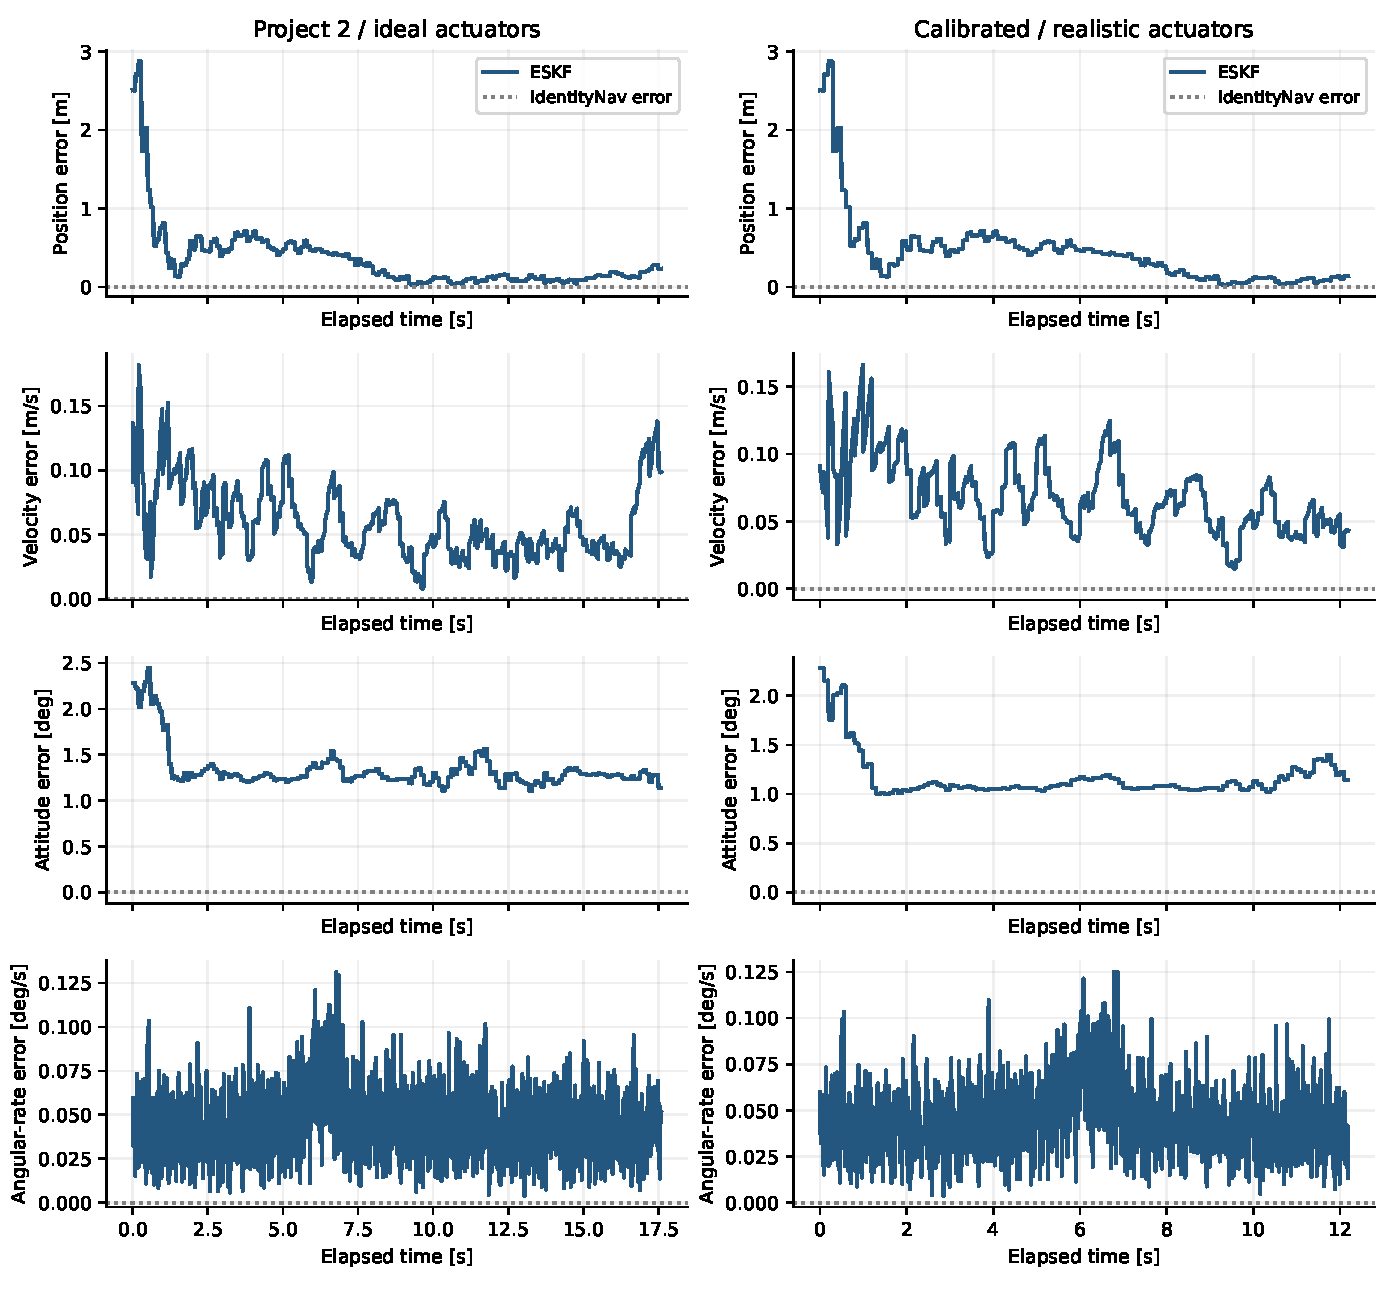
\includegraphics[width=\textwidth,height=0.72\textheight,keepaspectratio]{report_assets/navigation_closed_loop.pdf}
\caption{ESKF position, velocity, attitude, and angular-rate error norms in the two
closed-loop cases. Dotted zero lines indicate ideal-feedback estimation error.
Each ESKF history is compared with its own plant truth.}\label{fig:nav-closed-loop}
\end{figure}

\begin{figure}[!htbp]\centering
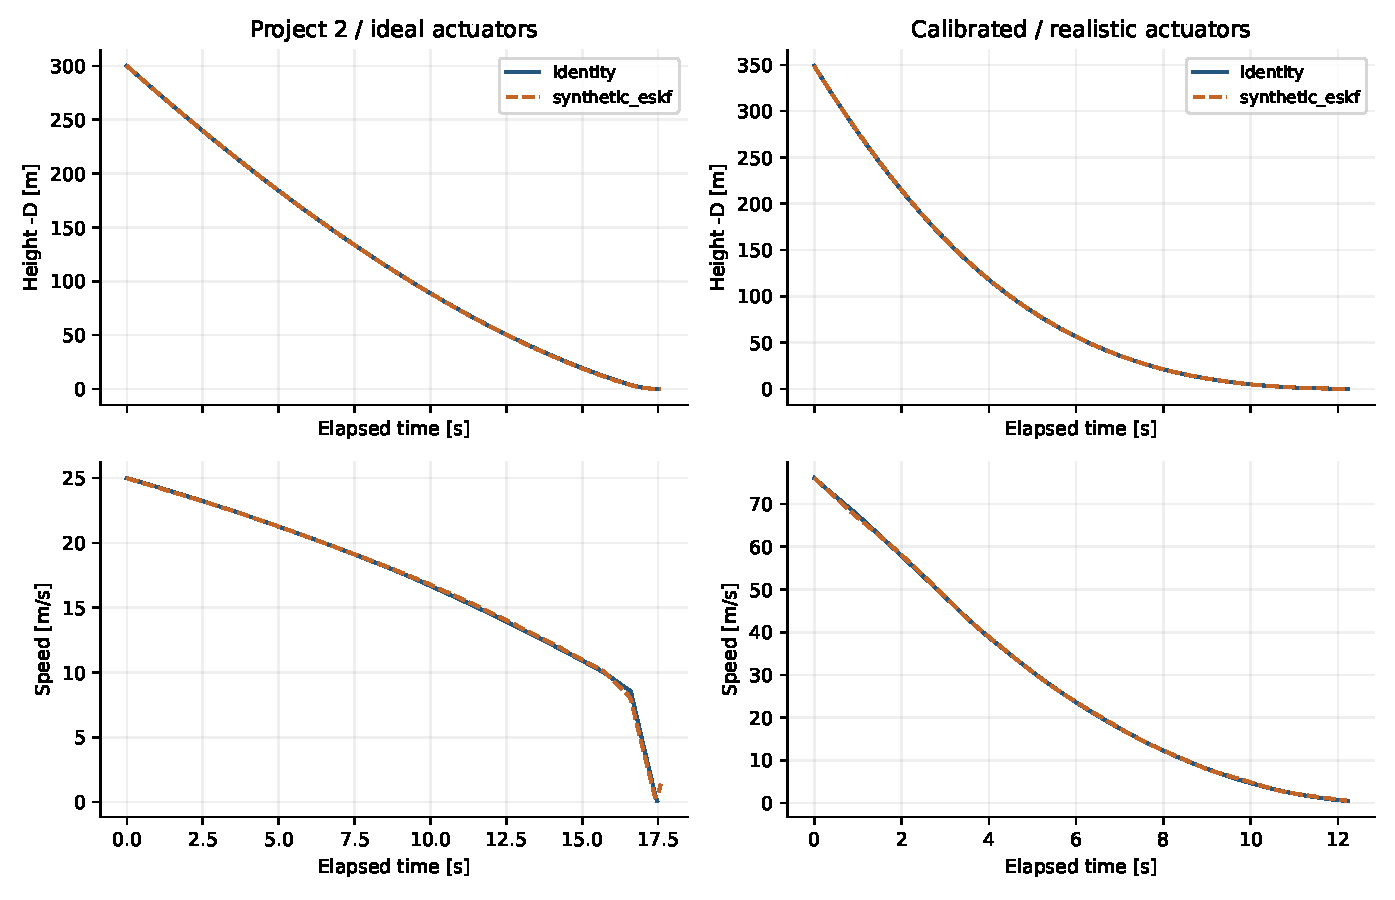
\includegraphics[width=\textwidth,height=0.58\textheight,keepaspectratio]{report_assets/navigation_landing.pdf}
\caption{True height and speed under identity and ESKF feedback. The height curves use
the near-pad tangent height $-r_D$; contact metrics use radial altitude.
Each panel retains its scenario's plant and controller settings.}\label{fig:nav-landing}
\end{figure}

\subsection{Fixed-Trajectory Filter Comparison and GNSS Outage}\label{sec:nav-replay}

To isolate estimation from changing closed-loop trajectories, the calibrated identity
run's truth is replayed at 100 Hz. Native CG force and inertial-rate histories are recorded at every navigation epoch.
One sensor generator uses these histories to create a common sample sequence; each filter receives an independent copy of the same measurements. Three cases
share the same GNSS/radar initialization and uncertain alignment observation: IMU-only propagation
with all subsequent aiding disabled, the nominal ESKF, and an ESKF with GNSS updates
suppressed from 4 through 8 s while radar remains available. The replay has 1,223 IMU
samples over 0--12.22 s, 121 valid nominal GNSS updates, and 245 radar samples. Suppressing
the selected interval leaves 80 GNSS updates. No replay estimate is fed back into the plant.

\begin{table}[!htbp]\centering\small
\caption{RMSE on identical truth and sensor samples. The IMU-only case retains the common
initial aided update and then propagates without further GNSS or radar corrections.}
\label{tab:nav-replay}
\begin{tabularx}{\textwidth}{l*{4}{>{\raggedleft\arraybackslash}X}}\toprule
Replay case & Position [m] & Velocity [m/s] & Attitude [deg] & Rate [deg/s]\\\midrule
IMU only & 19.732 & 4.307 & 2.318 & 0.044\\
ESKF & 0.641 & 0.075 & 1.091 & 0.049\\
ESKF + GNSS outage & 0.756 & 0.068 & 1.114 & 0.045\\
\bottomrule\end{tabularx}

\end{table}
\FloatBarrier

GNSS/radar aiding reduces position RMSE from 19.732 to 0.641 m and velocity RMSE from
4.307 to 0.075 m/s. A four-second GNSS outage increases position RMSE to 0.756 m; radar
continues to constrain height. The slight decrease in aggregate velocity RMSE during this
particular outage is not evidence that discarding GNSS is beneficial. It is one finite
noise realization, and the horizontal and vertical channels have different aiding.

With uncertain initial alignment, attitude RMSE decreases from 2.318 deg in IMU-only
propagation to 1.091 deg with ESKF aiding. Angular-rate RMSE is 0.044 deg/s and
0.049 deg/s, respectively: aiding does not reduce every error metric. The short,
nearly vertical trajectory has no direct attitude observation after initialization.
Figure~\ref{fig:nav-biases} shows that not every bias component converges; the longer
ascent and consistency experiments below examine a wider excitation and time range.

\begin{figure}[!htbp]\centering
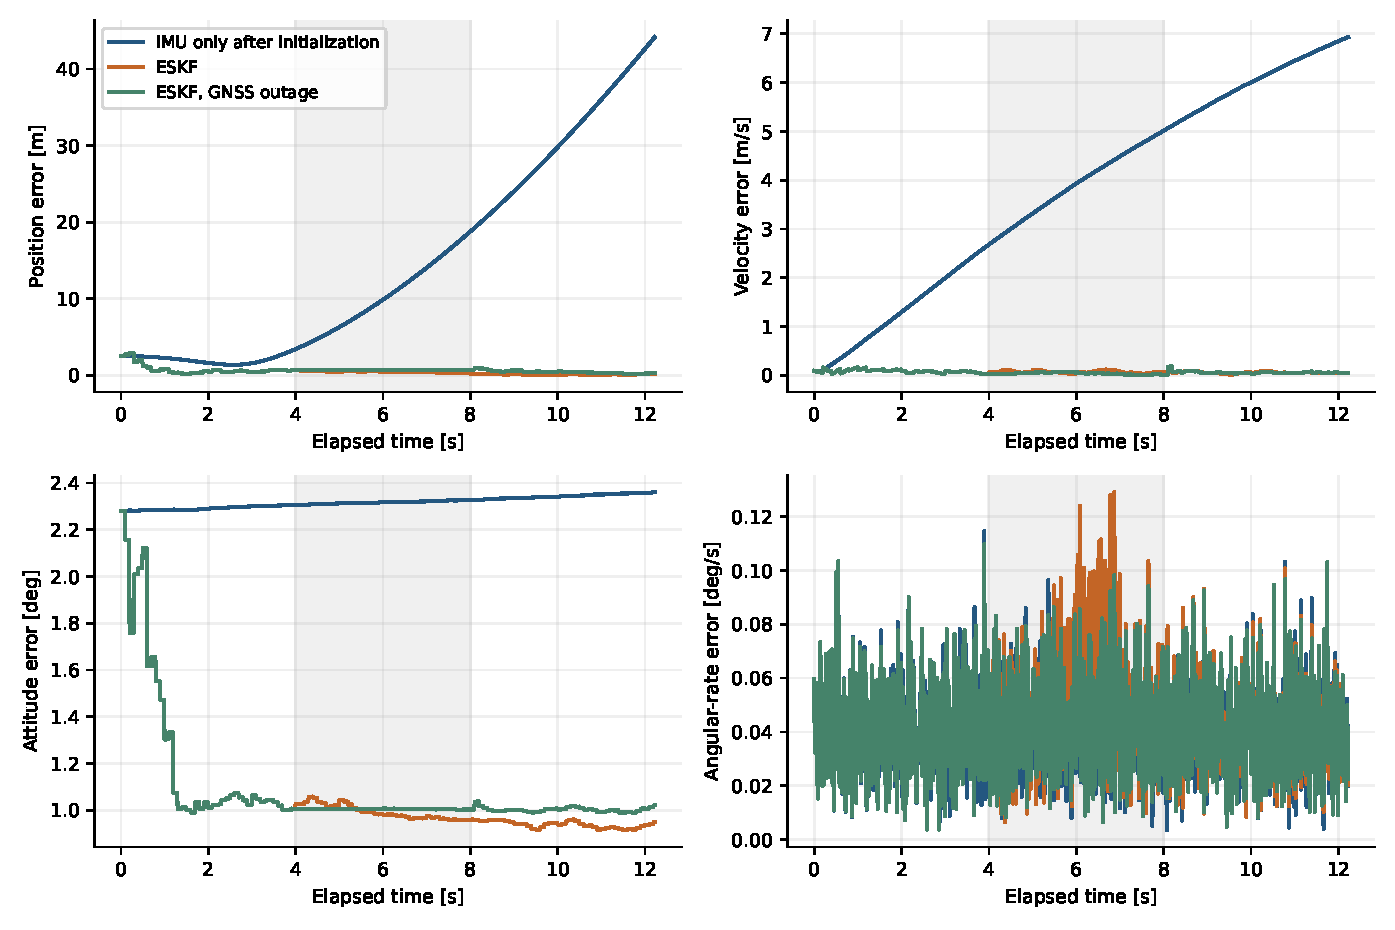
\includegraphics[width=\textwidth,height=0.60\textheight,keepaspectratio]{report_assets/navigation_replay.pdf}
\caption{Fixed-truth replay comparison. The shaded interval is the GNSS outage applied
only to the outage variant; radar remains active. All three cases receive the same IMU
samples and start from the same nominal state and covariance.}\label{fig:nav-replay}
\end{figure}

\begin{figure}[!htbp]\centering
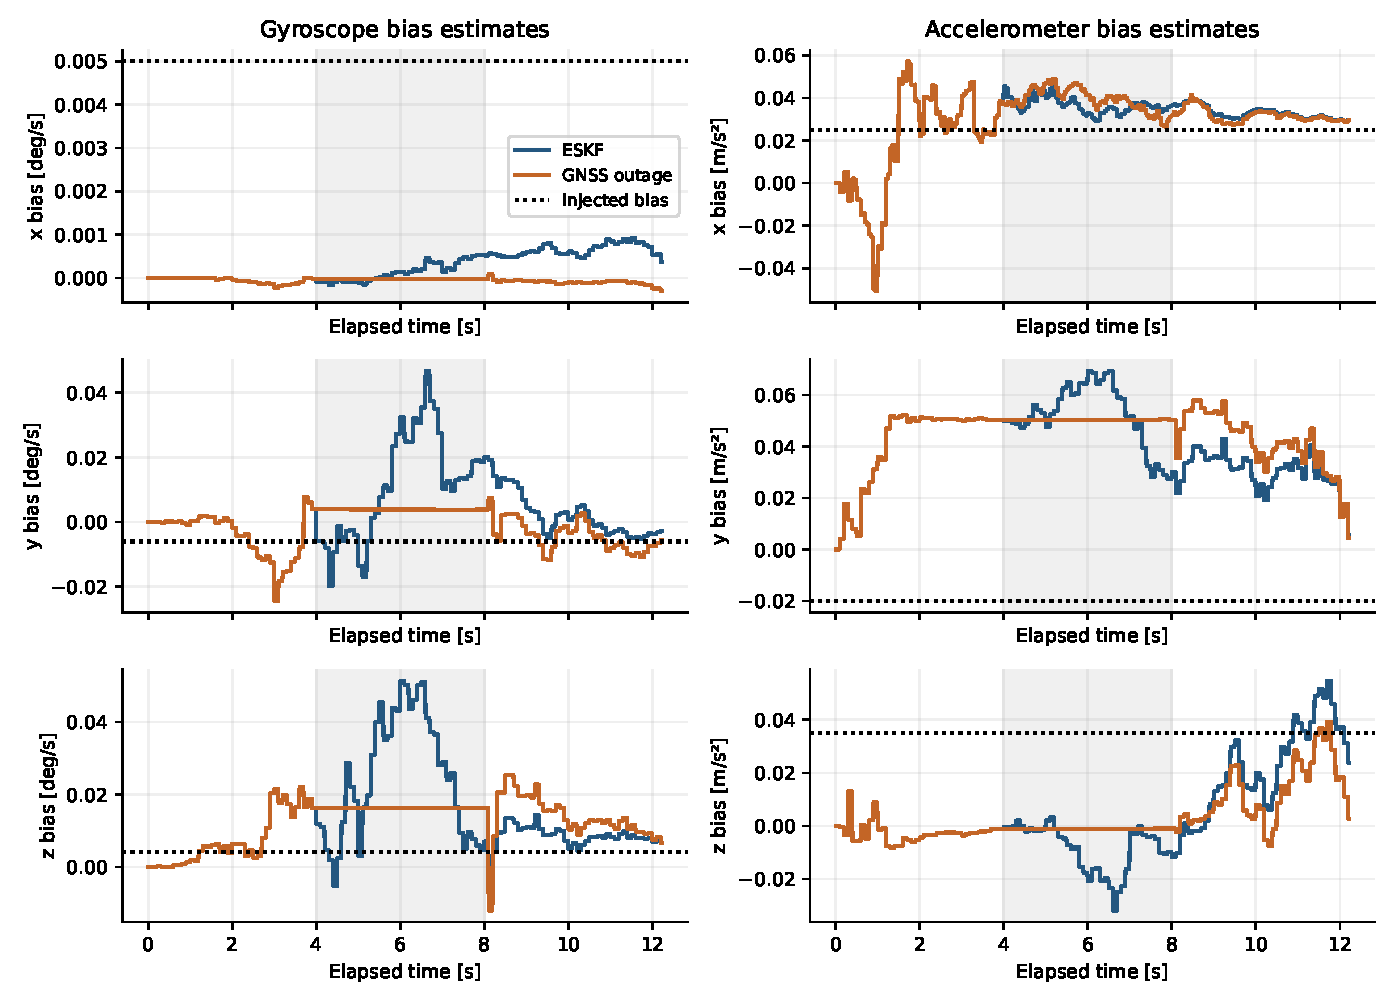
\includegraphics[width=\textwidth,height=0.63\textheight,keepaspectratio]{report_assets/navigation_biases.pdf}
\caption{Estimated IMU biases in fixed-truth replay, with the constant injected biases
shown as dotted lines. The short experiment does not show convergence of every bias
component. The shaded interval suppresses GNSS only in the outage variant.}\label{fig:nav-biases}
\end{figure}

\FloatBarrier
\subsection{Multiple Seeds and Missing-GNSS Startup}\label{sec:nav-robustness}
Each landing scenario is repeated with seeds 0--9, a 1 deg per-axis initial alignment
uncertainty, and the same sensor parameters and unchanged controller settings. A third
condition uses the Project~2 landing with GNSS suppressed from 0 through 3 s. Its declared
initial position prior has offset $(10,-8,5)$ m and velocity prior has offset
$(0.5,-0.4,0.3)$ m/s; radar remains available. Thus the prior is deliberately different
from truth, and the estimator must propagate and acquire GNSS after startup.
\begin{table}[!htbp]\centering\small
\caption{Ten-seed closed-loop evaluation per condition. Maxima include unsuccessful runs;
mean position RMSE is the arithmetic mean of the ten per-run RMSEs.}\label{tab:nav-seeds}
\begin{tabularx}{\textwidth}{Yrrrr}\toprule
Case & Soft success & Max speed [m/s] & Max miss [m] & Mean pos. RMSE [m]\\\midrule
Project 2 & 5/10 & 6.539 & 1.152 & 0.539\\
Calibrated & 10/10 & 1.314 & 1.836 & 0.615\\
Project 2, startup outage & 4/10 & 4.444 & 4.358 & 5.973\\
\bottomrule\end{tabularx}

\end{table}
\FloatBarrier
The calibrated realistic-actuator case succeeds in all ten runs. The original Project~2
configuration succeeds in five; with the startup outage and perturbed prior it succeeds
in four. The nominal Project~2 maximum contact speed is 6.539 m/s despite a mean
position-estimation RMSE of 0.539 m. These outcomes show that the original ideal-actuator
landing configuration is sensitive to state-estimation errors. Successful initialization
and sub-metre average estimation error do not guarantee a soft landing. The empirical
counts describe these finite trials, not a qualified flight success probability; no
controller gains were changed to improve the counts. The two scenario families differ in
initial condition, vehicle and guidance settings, so their success counts do not isolate
the effect of actuator fidelity.

\subsection{Long Ascent Replay and Covariance Diagnostics}\label{sec:nav-consistency}
The native 150-second \texttt{project2\_ascent} trajectory is recorded at 100 Hz,
including its 10--12 s gimbal maneuver, throttle changes, cutoff at 145 s, and coast.
The physical IMU channels come directly from native loads and inertial angular rates.
Five seeds (0--4) are replayed under three conditions: nominal aiding, no GNSS from
0 through 5 s, and no GNSS from 60 through 80 s. The startup case uses the same nonzero
prior offsets as the landing test. All variants within each seed receive identical
sensor samples and alignment observation; only GNSS availability and the startup
initialization differ. Radar follows the 1500 m range limit and cannot aid the
high-altitude 20-second outage. Estimates are not fed back into this prescribed ascent.
\begin{table}[!htbp]\centering\small
\caption{Five-seed 150-second ascent replay. RMSE columns are means of per-run RMSEs;
NEES is averaged over the five seeds and all sampled epochs.}\label{tab:nav-ascent}
\begin{tabularx}{\textwidth}{Yrrrr}\toprule
Ascent case & Pos. RMSE [m] & Vel. RMSE [m/s] & Att. RMSE [deg] & Mean NEES\\\midrule
Nominal & 0.380 & 0.054 & 0.750 & 10.70\\
Startup outage (5 s) & 2.833 & 0.262 & 0.866 & 10.83\\
In-flight outage (20 s) & 1.059 & 0.143 & 0.933 & 11.17\\
\bottomrule\end{tabularx}

\end{table}
\FloatBarrier
All startup-outage runs acquire GNSS at 5.1 s. Initial attitude-error magnitudes range
from 0.703 to 2.332 deg. Across the fifteen ascent replays, final position-error magnitude
is at most 0.414 m and final attitude error at most 0.715 deg. The nominal mean position
RMSE is 0.380 m; the startup and in-flight outages increase it to 2.833 and 1.059 m.
The maximum transient position errors are 23.389 m and 8.664 m in the two outage
conditions. These results demonstrate recovery after aiding returns, rather than
continuous nominal accuracy during the outages.

The full 15-state normalized estimation error squared and measurement normalized
innovation squared are
\begin{equation}
 \mathrm{NEES}_k=\bm e_k^TP_k^{-1}\bm e_k,\qquad
 \mathrm{NIS}_k=\bm y_k^TS_k^{-1}\bm y_k,
\end{equation}
where $\bm e$ includes position, velocity, global attitude error, and both bias errors.
For five independent seeds, the reference pointwise 95\% band for mean NEES is
$[10.588,20.168]$, obtained from a chi-square distribution with 75 degrees of freedom.
Mean GNSS NIS is 5.995--6.007 (six measurement components), and mean altimeter NIS is
0.992--0.997 (one component). However, only 50.4--59.0\% of epochs have ensemble NEES
inside the reference band. Thus measurement innovations have appropriate mean scale
in these tests, while full-state covariance consistency is not established. The fixed
injected biases are not sampled from the complete Gaussian prior, process bias noise
allows variation absent from truth, and temporal samples are correlated. The band is a
diagnostic reference, not a sequence of independent acceptance tests or a reason to
retune covariance until a desired pass fraction is obtained.
\begin{figure}[!htbp]\centering
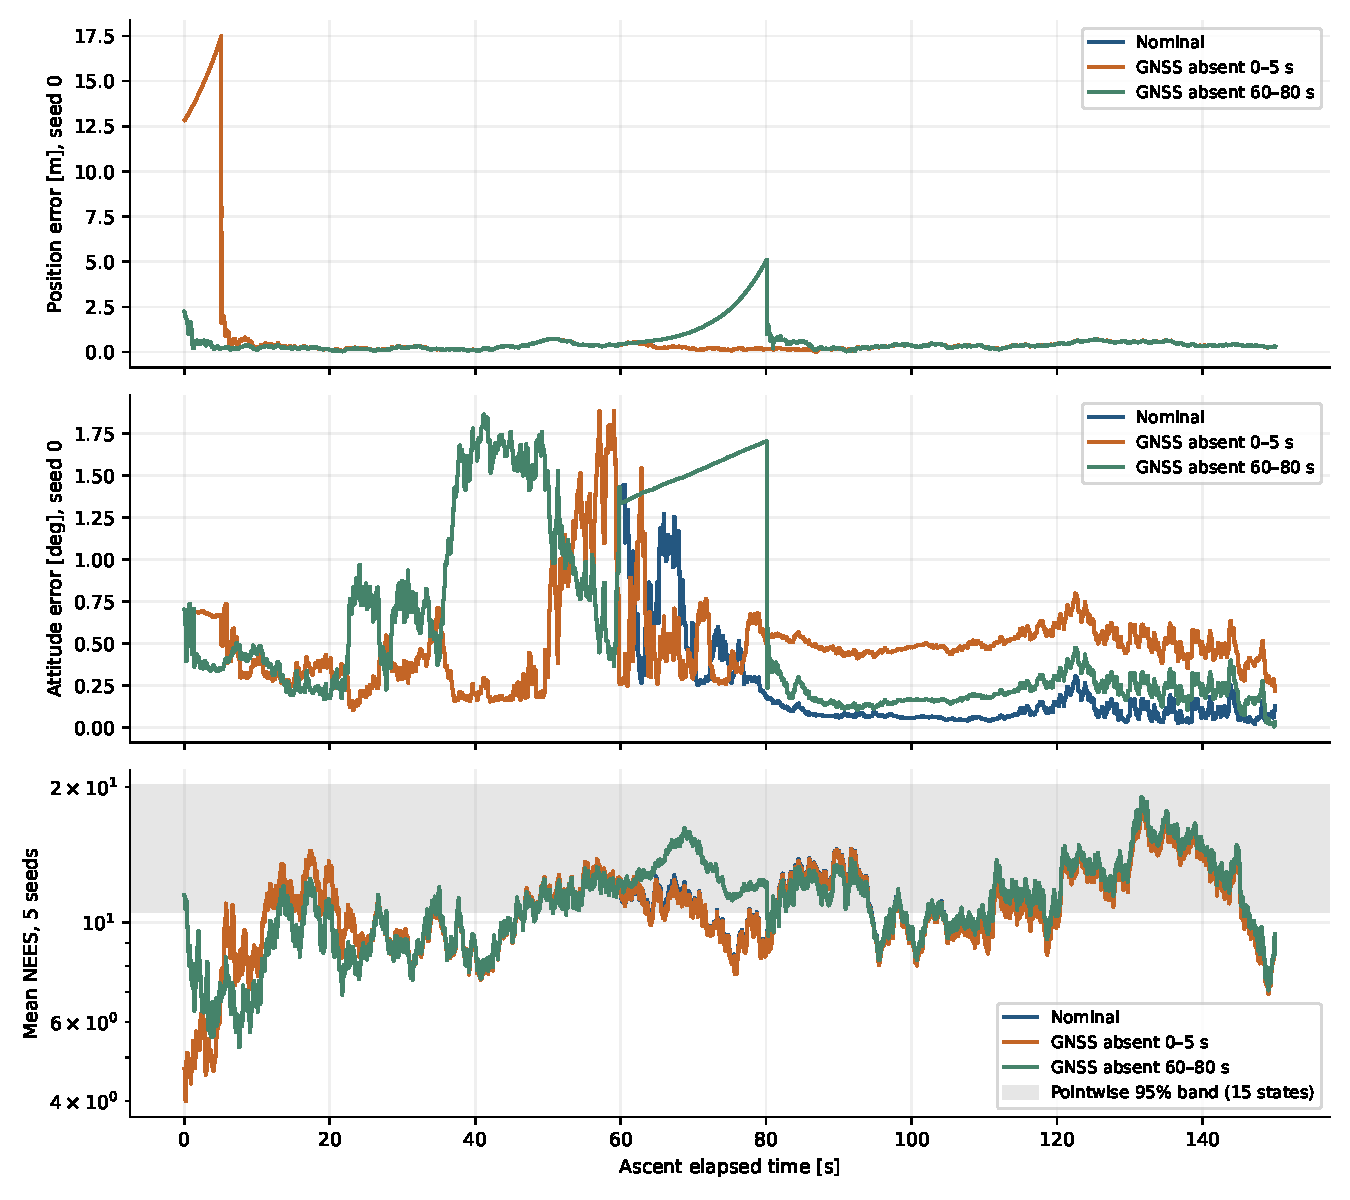
\includegraphics[width=\textwidth,height=0.72\textheight,keepaspectratio]{report_assets/navigation_robustness.pdf}
\caption{Native ascent replay: seed-0 position and attitude error, and five-seed mean NEES.
The pointwise consistency band is shown for the 15-state error.}\label{fig:nav-robustness}
\end{figure}
\FloatBarrier

\subsection{Verification Scope and Remaining Navigation Limitations}\label{sec:nav-limits}
Physical checks cover zero accelerometer output in vacuum free fall, pad support,
Earth-rate gyro output, and drift-free noiseless propagation at an Earth-fixed point
away from the reference origin. Finite differences verify the radial-height/gravity
Jacobians and global attitude reset. Initialization tests exercise absent GNSS,
nonzero alignment error, and single use of the first GNSS sample. Replay checks include
finite estimates, quaternion normalization, and covariance positivity. Additional checks
verify optional scale-factor/random-walk inputs, explicit sensor-rate validation, GNSS
outlier rejection, and common uncertain initialization of the IMU-only and aided estimators.

The expanded study evaluates small unknown alignment errors, delayed GNSS acquisition,
multiple seeds, and longer high-altitude outages. It does not establish autonomous
alignment from an arbitrary unknown attitude, hardware sensor accuracy, global
covariance consistency, or robust landing over the full operating envelope. Mass remains
an ideal auxiliary measurement. The sensors omit latency, lever arms, saturation, and
vibration; the altimeter assumes radial height. These technical limits remain relevant
to guidance and control design even when the filter is numerically well behaved.


\section{Discussion and Limitations}\label{sec:discussion}
\subsection{Interpretation and Applicability of the Results}
The verification results support the implementation of the declared equations within the tested regimes. The phase experiments reproduce expected mechanisms: propellant depletion and acceleration during ascent, powered deceleration during entry and terminal descent, and drag-driven deceleration with constant mass during aerodynamic descent. The landing experiment additionally demonstrates nominal feedback control under its selected initial condition and ideal actuator assumptions.

Flight agreement is substantially weaker than numerical agreement. In particular, the ascent residual prevents treating the baseline as a quantitatively validated CRS-11 predictor. Recovery intervals begin from separately prescribed states, so their errors do not include the accumulated uncertainty of earlier phases. The assumed latitude, heading, and horizontal origins also preclude a geographic landing-site reconstruction. No landing robustness probability follows from a single nominal successful case.

\subsection{Model Uncertainties and GNC Design Risks}
The most consequential errors depend on flight phase. During low-altitude braking, effective thrust and actuator delay affect stopping distance and available fuel margin. Using ideal actuation can hide insufficient time to build thrust or redirect the vehicle. Aerodynamic forces and moments dominate atmospheric descent; uncertainty in coefficients, wind, and CG can shift both the terminal state and available control authority. During final approach, state-estimation errors can cause the controller to satisfy constraints for the wrong state.
\begin{table}[!htbp]
\centering\small
\caption{Priority uncertainties for subsequent GNC design.}\label{tab:risks}
\begin{tabularx}{\textwidth}{>{\raggedright\arraybackslash}p{0.19\textwidth}YY}\toprule
Uncertainty & Consequence & Next evaluation\\\midrule
Navigation bias, delay, dropout & Incorrect burn timing, attitude commands, or perceived touchdown state & Wider alignment/bias/latency dispersions and covariance calibration\\
Thrust and actuator response & Late braking, saturation, excessive fuel use & Thrust-bias and response-delay sweeps with realistic actuation\\
Aerodynamic loads and wind & Entry load error and displaced landing initial state & Coefficient/wind dispersions across the tested Mach and pressure range\\
Mass, CG, inertia & Incorrect acceleration and control-moment prediction & Coupled mass-property perturbations and allocation checks\\
Frame or altitude mismatch & Persistent sensor, guidance, or contact error & Explicit inertial/Earth-relative transformations and common altitude datum\\\bottomrule
\end{tabularx}
\end{table}

Navigation uncertainty and realistic thrust response are absent from the original nominal landing baseline. The extension evaluates ESKF feedback in both ideal- and realistic-actuator landing scenarios, with changed contact performance despite successful seed-0 landings. Across ten seeds, the original configuration succeeds in five cases and the calibrated configuration in ten; the startup-outage variant of the original configuration succeeds in four. Broader sensor and actuator uncertainty remains important for qualification. For atmospheric descent, the large modeled pressure peak makes aerodynamic and structural assumptions a separate priority. These priorities follow the mechanisms exercised here; their relative quantitative severity has not yet been ranked by a common sensitivity study.

\subsection{Remaining Work}
The navigation study includes native-force IMU measurements, rotating-frame propagation, uncertain alignment, and missing-GNSS initialization. Remaining work includes hardware-based sensor parameters, autonomous alignment without an external attitude prior, bias observability, and covariance calibration under wider flight conditions. The physical-model program should extend the separately identified calibration work and realistic-actuator case with independent data and parameter dispersions, while retaining the original comparison as a baseline. Aerodynamic data quality, upper-atmosphere continuation, Earth oblateness, and landing-impact dynamics define additional fidelity limits.

\section{Conclusions}
The simulator couples translational and rotational motion, variable mass properties, propulsion, aerodynamics, and rotating-Earth effects in a common execution framework. Four prescribed-input experiments and one closed-loop landing case demonstrate distinct ascent and recovery mechanisms. The selected archived reference comparisons agree within the stated numerical tolerances, and the nominal landing reaches contact with approximately \SI{0.086}{\metre\per\second} speed under ideal actuation.

Public-flight comparison exposes limitations that numerical verification cannot resolve. The ascent altitude RMSE of \SI{10.72}{\kilo\metre} and the recovery residuals require investigation of physical parameters and input histories before using the baseline for quantitative flight prediction. The synthetic sensor-and-ESKF extension demonstrates sensor-based closed-loop operation and quantifies state-estimation errors; its multi-seed landing and ascent experiments quantify initialization and outage sensitivity, with the remaining sensor and statistical limitations stated explicitly. The current results establish a reproducible model-development baseline; extending it to GNC design requires the uncertainty and feedback evaluations identified in Section~\ref{sec:discussion}.

\clearpage
\begin{thebibliography}{9}
\raggedright
\addcontentsline{toc}{section}{References}
\bibitem{ussa} NOAA, NASA, and USAF, \emph{U.S. Standard Atmosphere, 1976}, NOAA-S/T-76-1562, NASA-TM-X-74335, October 1976. \url{https://ntrs.nasa.gov/citations/19770009539}.
\bibitem{telemetry} shahar603, \emph{Telemetry-Data: SpaceX CRS-11, stage-1 raw data}, commit \code{b245d3b81aa36b7941ec10f3f4b508999d106a6d}, local snapshot retrieved 2 November 2026. \url{https://github.com/shahar603/Telemetry-Data/tree/b245d3b81aa36b7941ec10f3f4b508999d106a6d/SpaceX%20CRS-11/JSON}.
\bibitem{sola} J. Sol\`a, \emph{Quaternion kinematics for the error-state Kalman filter}, 2017. \url{https://arxiv.org/abs/1711.02508}.
\end{thebibliography}

\appendix
\clearpage
\section{Reproduction Guide}\label{app:reproduction}
\subsection{Evidence Selection and File Integrity}
The original physics and flight-comparison figures use \path{results/verification/project2_segments/physics/<case>/physics.npz}. The navigation figures use the separate new campaign described in Section~\ref{sec:nav-reproduction}. The accompanying \path{resolved_config.yaml}, \path{verification.json}, and, for prescribed cases, \path{convergence.json} define the campaign and checks. Table~\ref{tab:runs} identifies the selected runs; the date is taken from the recorded run IDs. Contact metrics also use \path{results/project2_physics/landing/kpi.json}, whose speed, position-error, and tilt fields were cross-checked against the landing verification record.
\begin{table}[!htbp]
\centering\small\caption{Archived run identifiers used in this report.}\label{tab:runs}
\begin{tabular}{ll}\toprule Case & Run ID\\\midrule
Ascent & \code{single\_20261103\_232516}\\
Entry burn & \code{single\_20261103\_232531}\\
Aero descent & \code{single\_20261103\_232535}\\
Powered descent & \code{single\_20261103\_232543}\\
Landing & \code{single\_20261103\_232548}\\\bottomrule
\end{tabular}
\end{table}

The plotting script \path{report_assets/generate_figures.py} reads these histories without executing the plant or altering the stored results. It recomputes comparison statistics from the pinned raw observations and records SHA-256 hashes of input data, configurations, verification records, and processing sources in \path{report_assets/metrics.json}. This separates the archived simulation campaign from report-time post-processing. The latter was performed on 10 November 2026. The saved run configurations govern the numerical claims; changing the current source or configuration can change newly generated runs.

\subsection{Environment and Run Commands}
The project requires Python 3.10 or later and a C++ compiler. From the repository root, create an environment and install the editable package:
\begin{lstlisting}
python3 -m venv .venv
.venv/bin/python -m pip install -e ".[dev]"
\end{lstlisting}
The optional QOCO backend is installed with \code{.[dev,qoco]}; CLARABEL is included in the base dependencies. Record the installed package versions and source revision for new verification runs. A current-source run can be generated with:
\begin{lstlisting}
.venv/bin/python scripts/run_single.py scenario=project2_ascent hydra.run.dir=results/report_rerun/ascent
.venv/bin/python scripts/run_single.py scenario=project2_entry_burn hydra.run.dir=results/report_rerun/entry_burn
.venv/bin/python scripts/run_single.py scenario=project2_aero_descent hydra.run.dir=results/report_rerun/aero_descent
.venv/bin/python scripts/run_single.py scenario=project2_powered_descent hydra.run.dir=results/report_rerun/powered_descent
.venv/bin/python scripts/run_single.py scenario=project2_landing hydra.run.dir=results/report_rerun/landing
\end{lstlisting}
The checkers provide independent-reference, refinement, and rotating-Earth checks. Use separate output locations for a new campaign so that the selected records remain identifiable:
\begin{lstlisting}
.venv/bin/python scripts/check_project2_segments.py --output results/report_rerun/verification
.venv/bin/python scripts/check_rotating_earth.py --output results/report_rerun/rotating_earth
.venv/bin/python -m pytest tests/ -q
.venv/bin/ruff check src tests scripts
\end{lstlisting}
To regenerate the report's figures and comparison metrics from the selected archive and compile the document:
\begin{lstlisting}
.venv/bin/python report_assets/generate_figures.py
latexmk -pdf report.tex
\end{lstlisting}
Alternatively, \code{tectonic report.tex} produces the PDF with automatic bibliography and cross-reference passes. The archived result folders must be retained to regenerate the figures; the already generated figure PDFs suffice to compile this document.

\subsection{Navigation Campaign Reproduction}\label{sec:nav-reproduction}

The navigation results are newly executed runs, separate from the archived physics
campaign. From the repository root, regenerate the four paired closed-loop cases, the common-truth
replay, thirty additional landing trials, fifteen ascent replays, and the navigation figures/tables with:
\begin{lstlisting}
.venv/bin/python -m pip install -e ".[dev]"
.venv/bin/python report_assets/generate_navigation.py
.venv/bin/python -m pytest tests/test_synthetic_eskf.py tests/sim/test_timing_contract.py tests/sim/test_multirate.py tests/sim/test_flight_calibration.py -q
\end{lstlisting}
The generator writes resolved configurations, seed manifests, full-rate navigation
histories, physics histories, and contact/error summaries under
\path{results/report_navigation/}. The navigation histories include native specific force and inertial rate at the navigation period.
The fixed-truth replay additionally saves the actual
IMU/GNSS/radar samples, all estimator states, bias estimates, and covariance diagonals.
\path{report_assets/navigation_metrics.json} records source SHA-256 hashes, the base Git
revision, numerical package versions, data hashes, and the evaluation conventions. These records identify the evaluated source and environment.
The figures and generated numerical tables in \path{report_assets/navigation_*} are
included in the report source tree; the \path{results/} histories can be regenerated with the same command
or supplied with the results archive to inspect the complete time histories.

For a normal standalone run with replay and sensor post-processing:
\begin{lstlisting}
.venv/bin/python scripts/run_single.py scenario=flight_calibrated_landing gnc/navigation=synthetic_eskf hydra.run.dir=results/navigation_landing
\end{lstlisting}
Replacing \texttt{synthetic\_eskf} with \texttt{identity} selects exact state feedback.
The standalone runner's additional sensor CSVs are generated after the flight; the ESKF
has already used its online sensor model during the closed-loop simulation.

The IMU rate and navigation period are explicit and must agree; the report settings use
100 Hz and 10 ms. Neither runner changes the period automatically. An independent
same-truth comparison and diagnostic plots can also be generated with:
\begin{lstlisting}
.venv/bin/python scripts/analyze_navigation.py scenario=project2_landing
\end{lstlisting}
This optional comparison uses the same physical sensor and rotating-frame propagation.
Its seeded replay is separate from the online samples that influenced a closed-loop run.
Scale-factor, bias-random-walk, outlier and gate settings are optional experiments; the
nominal report configuration keeps them disabled.


\section{Detailed Scenario Parameters}\label{app:parameters}
\begin{table}[!htbp]
\centering\small
\caption{Mass budgets at initialization. Dry structure excludes both propellant systems.}\label{tab:massbudget}
\begin{tabularx}{\textwidth}{Yrrrr}\toprule
Case & Structure [kg] & Attached [kg] & Main propellant [kg] & RCS [kg]\\\midrule
Ascent & 25,000 & 120,000 & 400,000 & 200\\
Entry burn & 25,000 & 0 & 14,800 & 200\\
Aero descent & 25,000 & 0 & 8800 & 200\\
Powered descent & 25,000 & 0 & 6800 & 200\\
Landing & 25,600 & 0 & 3700 & 200\\\bottomrule
\end{tabularx}
\end{table}

The common oxidizer-to-fuel mass ratio is 2.56. Tank bottom positions measured from the respective body nose are $[-54,-68]$ m in ascent, $[-26,-40]$ m in the three recovery cases, and $[-22,-33]$ m in landing. Dry axial CG positions are $-58$, $-30$, and $-30$ m, respectively. The attached ascent component has axial CG $-14$ m and diagonal central inertia $[194400,7940000,7940000]~\si{\kilogram\metre\squared}$. The configured dry-structure inertia is $[43000,3700000,3700000]~\si{\kilogram\metre\squared}$. Tank inertia and parallel-axis terms are added during propagation.

Realistic throttle uses $\tau=\SI{0.25}{\second}$ and $r_u=\SI{1}{\per\second}$. TVC parameters are $\omega_n=\SI{37.7}{\radian\per\second}$, $\zeta=0.707$, and $r_\delta=\SI{0.35}{\radian\per\second}$; corresponding fin parameters are 18.8, 0.7, and 0.52 in the same units. TVC and fin command bounds are $\pm\SI{0.14}{\radian}$ and $\pm\SI{0.35}{\radian}$. These are command bounds; the damped servo model does not impose a rigid mechanical stop.

The analytic table uses base/transonic/hypersonic drag coefficients of $0.25/0.30/0.10$ in ascent and $1.0/0.9/0.8$ in recovery and landing. The incidence drag coefficient is 2.0 and normal-force slope parameter is 2.5. These values define the assumed parameterization, and should not be interpreted as measured coefficients. Complete scalar and array settings remain in the hashed resolved configurations.

\section{Supplementary Simulation and Verification Results}\label{app:supplement}
The following figures provide the attitude/rate, mass-property, and residual histories used to support the main interpretation. Body-axis tilt is the angle between $C_{BN}\bm e_x$ and radial upward direction. Body rates are Earth-relative and resolved in body axes. Flight-path angle is positive upward; the undefined zero-speed initial ascent value is left unplotted. Very-low-speed direction angles near landing should be interpreted together with the small dynamic pressure.
\reportfigure{attitude_rates}{Body-axis tilt, flight-path angle, and body angular rates for all five independently initialized cases. Quaternion-derived tilt avoids the singular Euler representation at vertical attitude.}{fig:attitude}
\reportfigure{mass_properties}{CG and diagonal inertia histories for ascent and entry burn. The ascent includes the attached upper assembly and uses a different nose origin; its absolute CG coordinates are not directly comparable with the recovery coordinates.}{fig:massprops}
\reportfigure{flight_residuals}{Simulation-minus-observation residuals at overlapping reference timestamps. The increasing ascent residual and intermediate aerodynamic-descent mismatch remain visible even when terminal values alone appear similar.}{fig:residuals}

\clearpage
\section{Simulator Replay Screenshots}\label{app:replay}
Figures~\ref{fig:replay-ascent-entry} and~\ref{fig:replay-descent} complement the landing view in Section~\ref{sec:replay}. They show the attached ascent configuration, engine activity during recovery burns, and exposed grid fins during descent. Where present, the amber dashed overlay combines webcast altitude with simulated horizontal positions; it is not a measured three-dimensional flight path. The screenshots retain the demonstration-run values described in Section~\ref{sec:replay}.

\begin{figure}[!htbp]
\centering
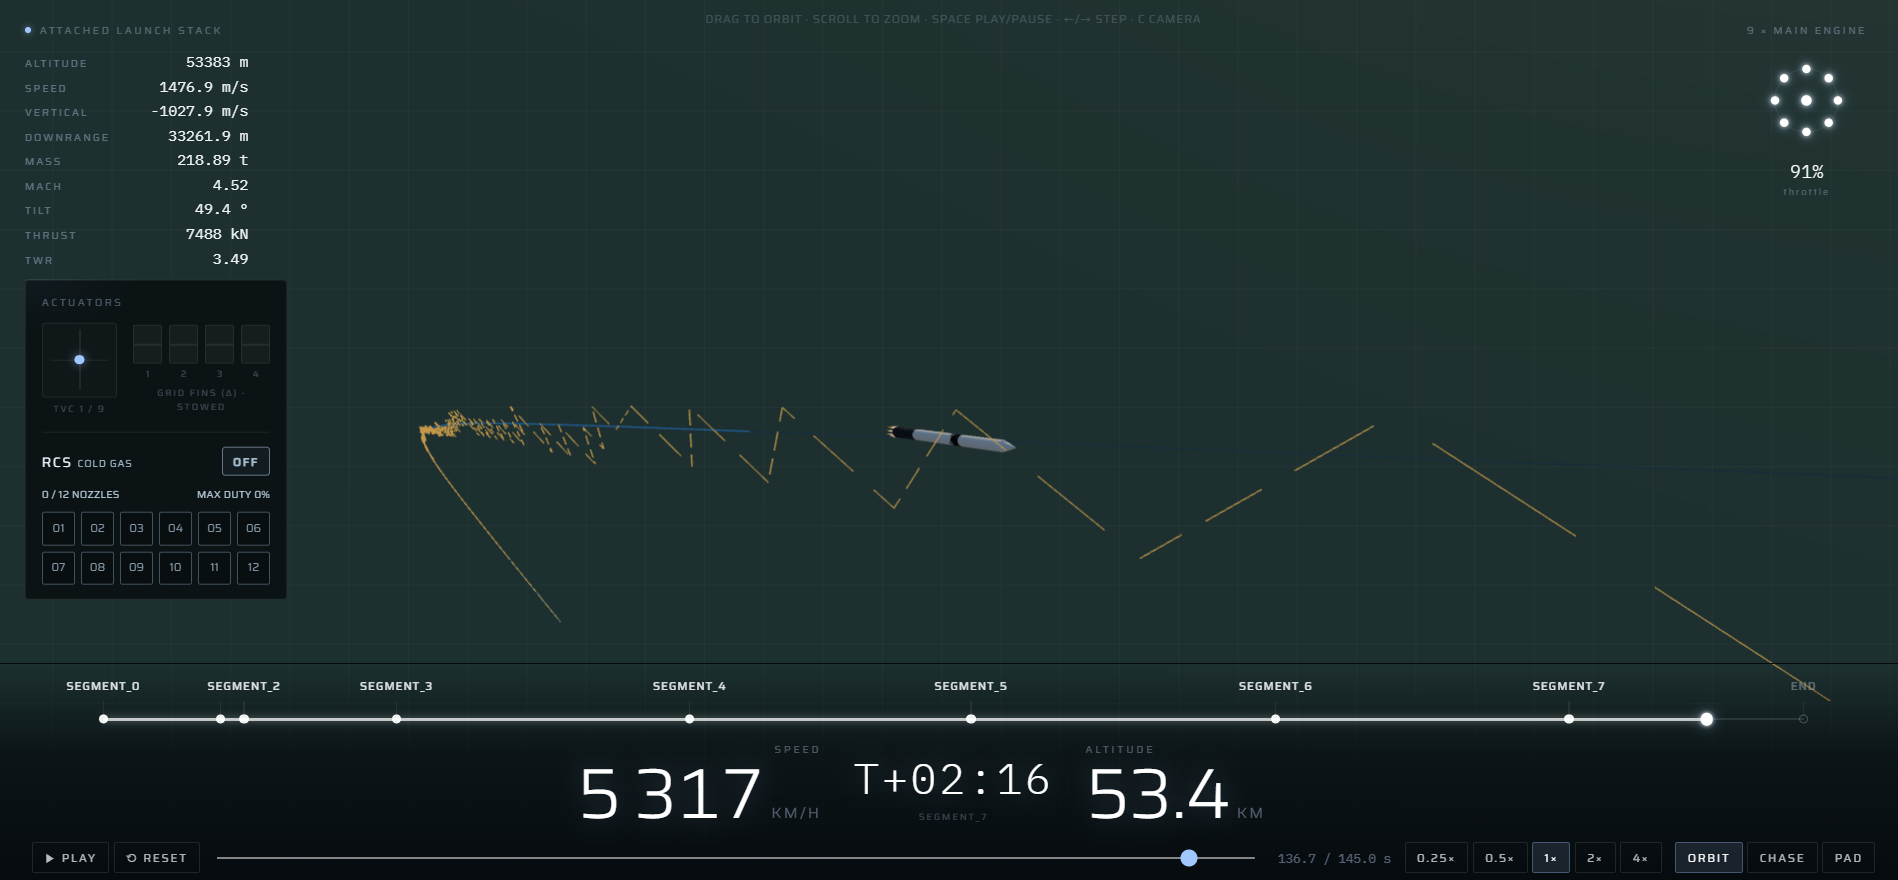
\includegraphics[width=\textwidth]{images/simulator_ascent.png}
\par\smallskip{\small (a) Powered ascent}\par\medskip
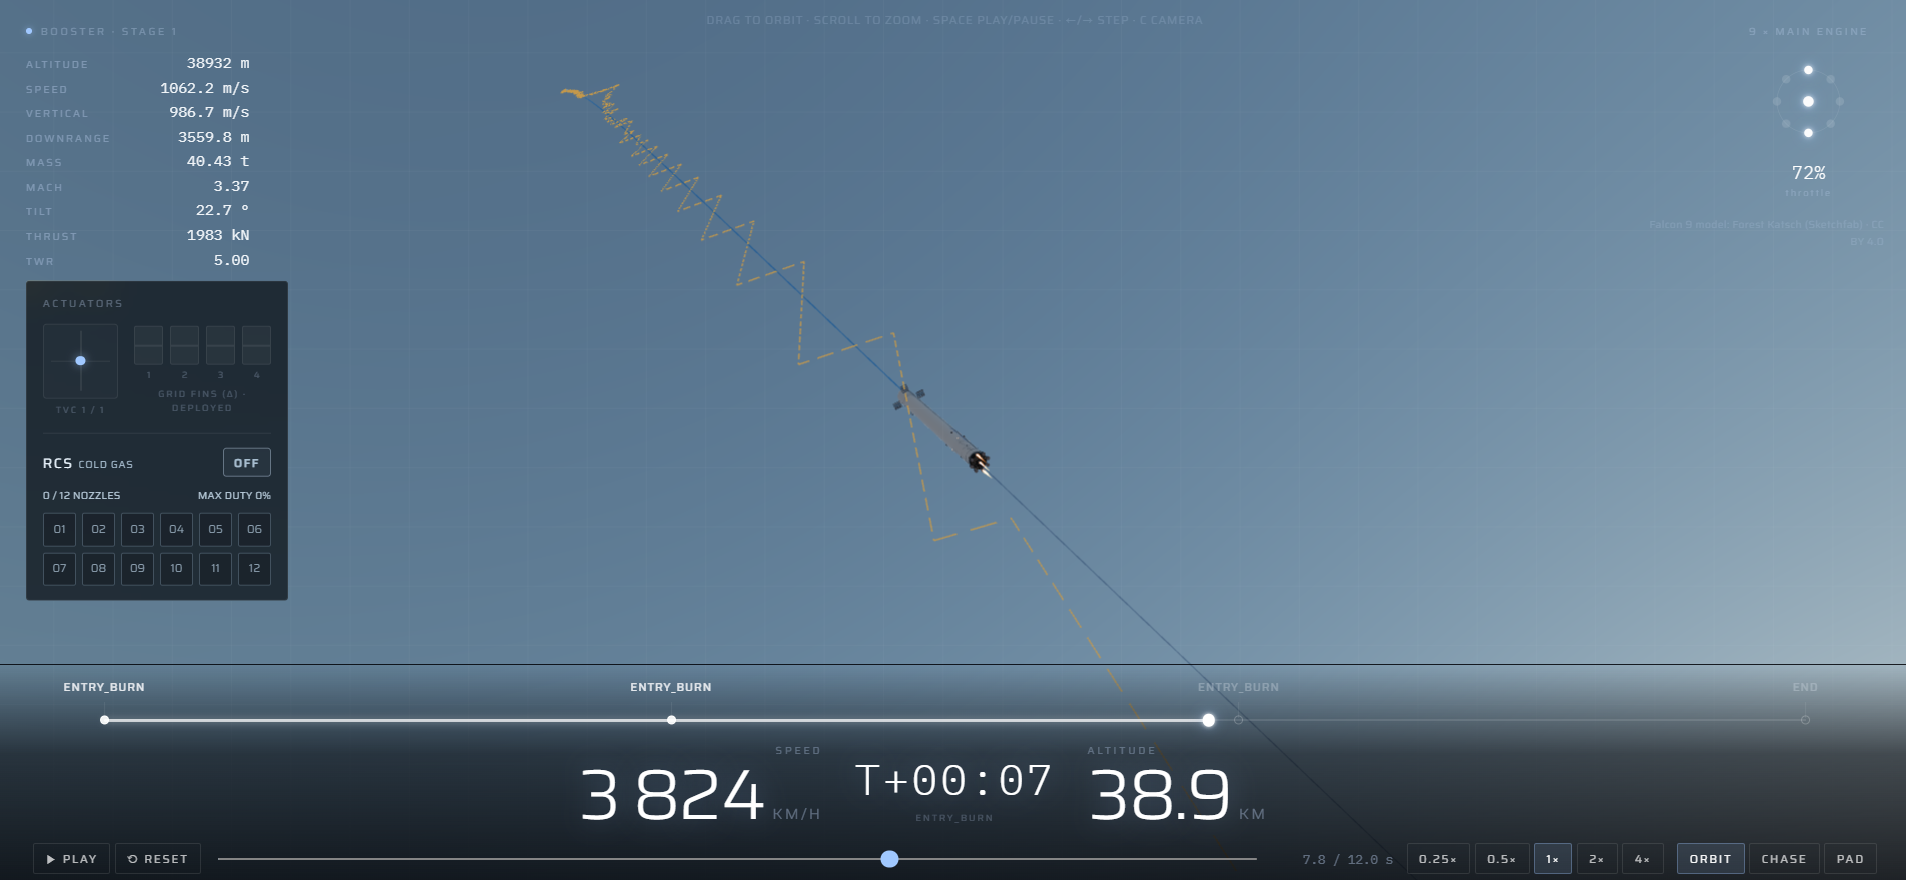
\includegraphics[width=\textwidth]{images/simulator_entry_burn.png}
\par\smallskip{\small (b) Entry burn}\par
\caption{Replay views of ascent and entry burn. The attached ascent stack has nine active engines and stowed fins; the recovery view shows three active engines and deployed fins. The timeline and telemetry panels allow the displayed geometry to be inspected alongside the recorded states. Recovery vehicle model: Forest Katsch (Sketchfab, CC BY 4.0).}
\label{fig:replay-ascent-entry}
\end{figure}
\FloatBarrier

\begin{figure}[!htbp]
\centering
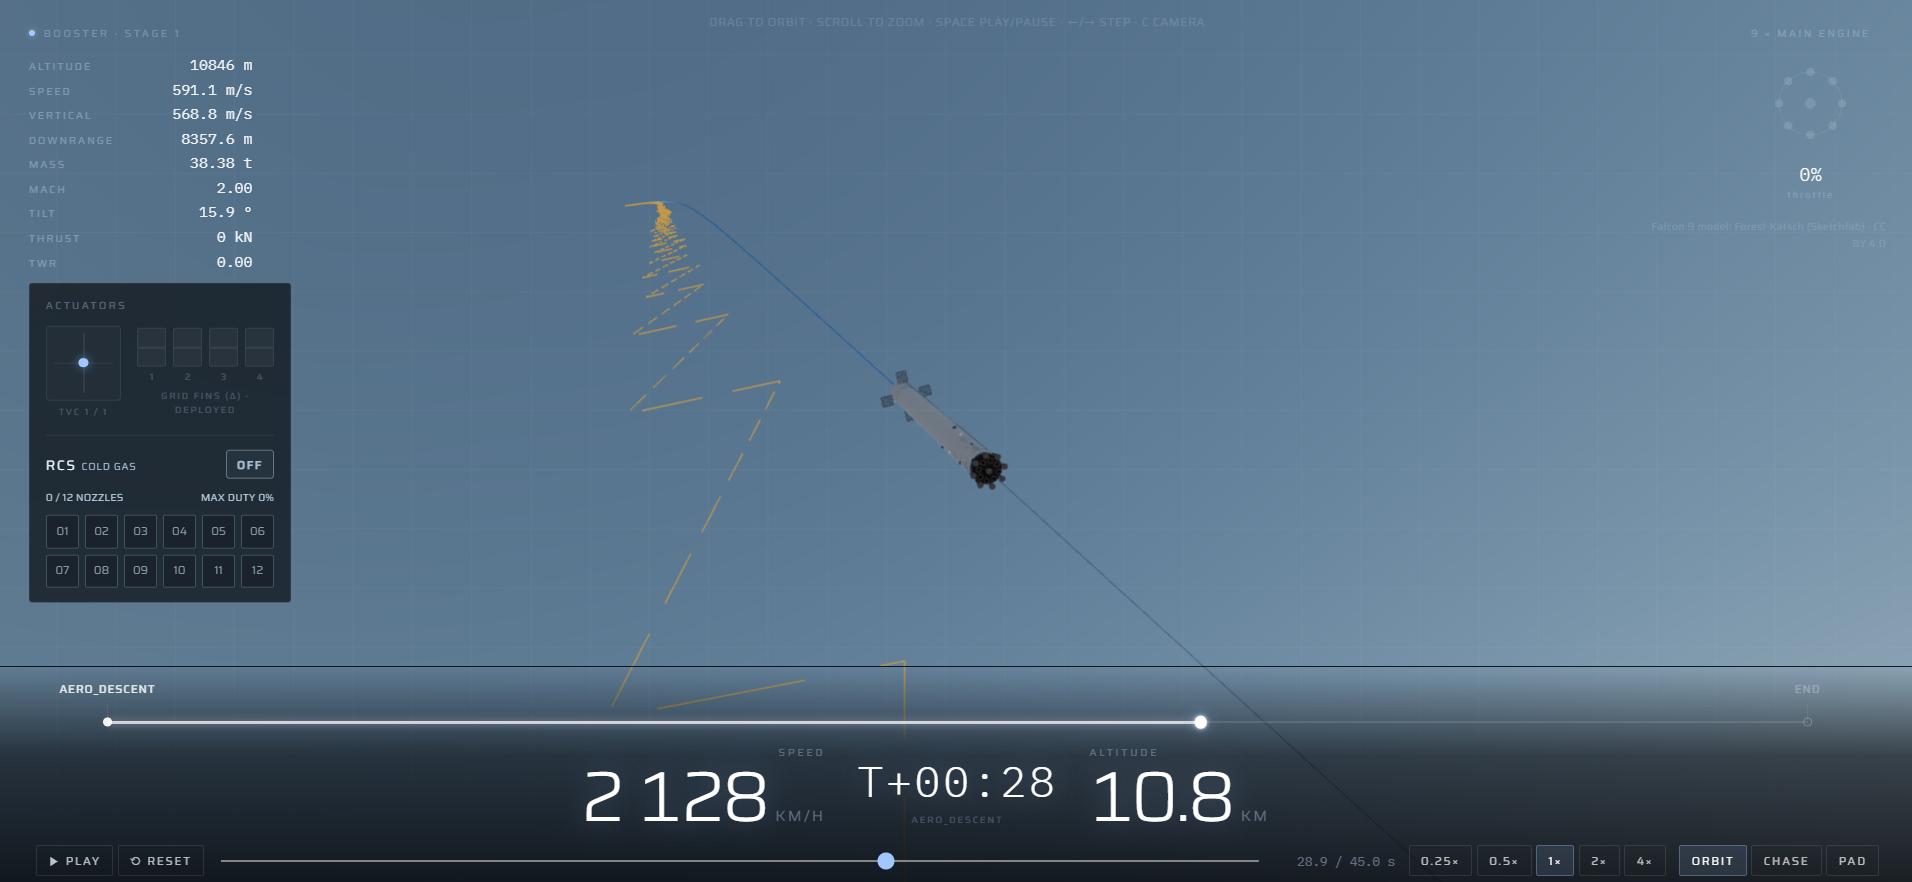
\includegraphics[width=\textwidth]{images/simulator_aero_descent.png}
\par\smallskip{\small (a) Aerodynamic descent}\par\medskip
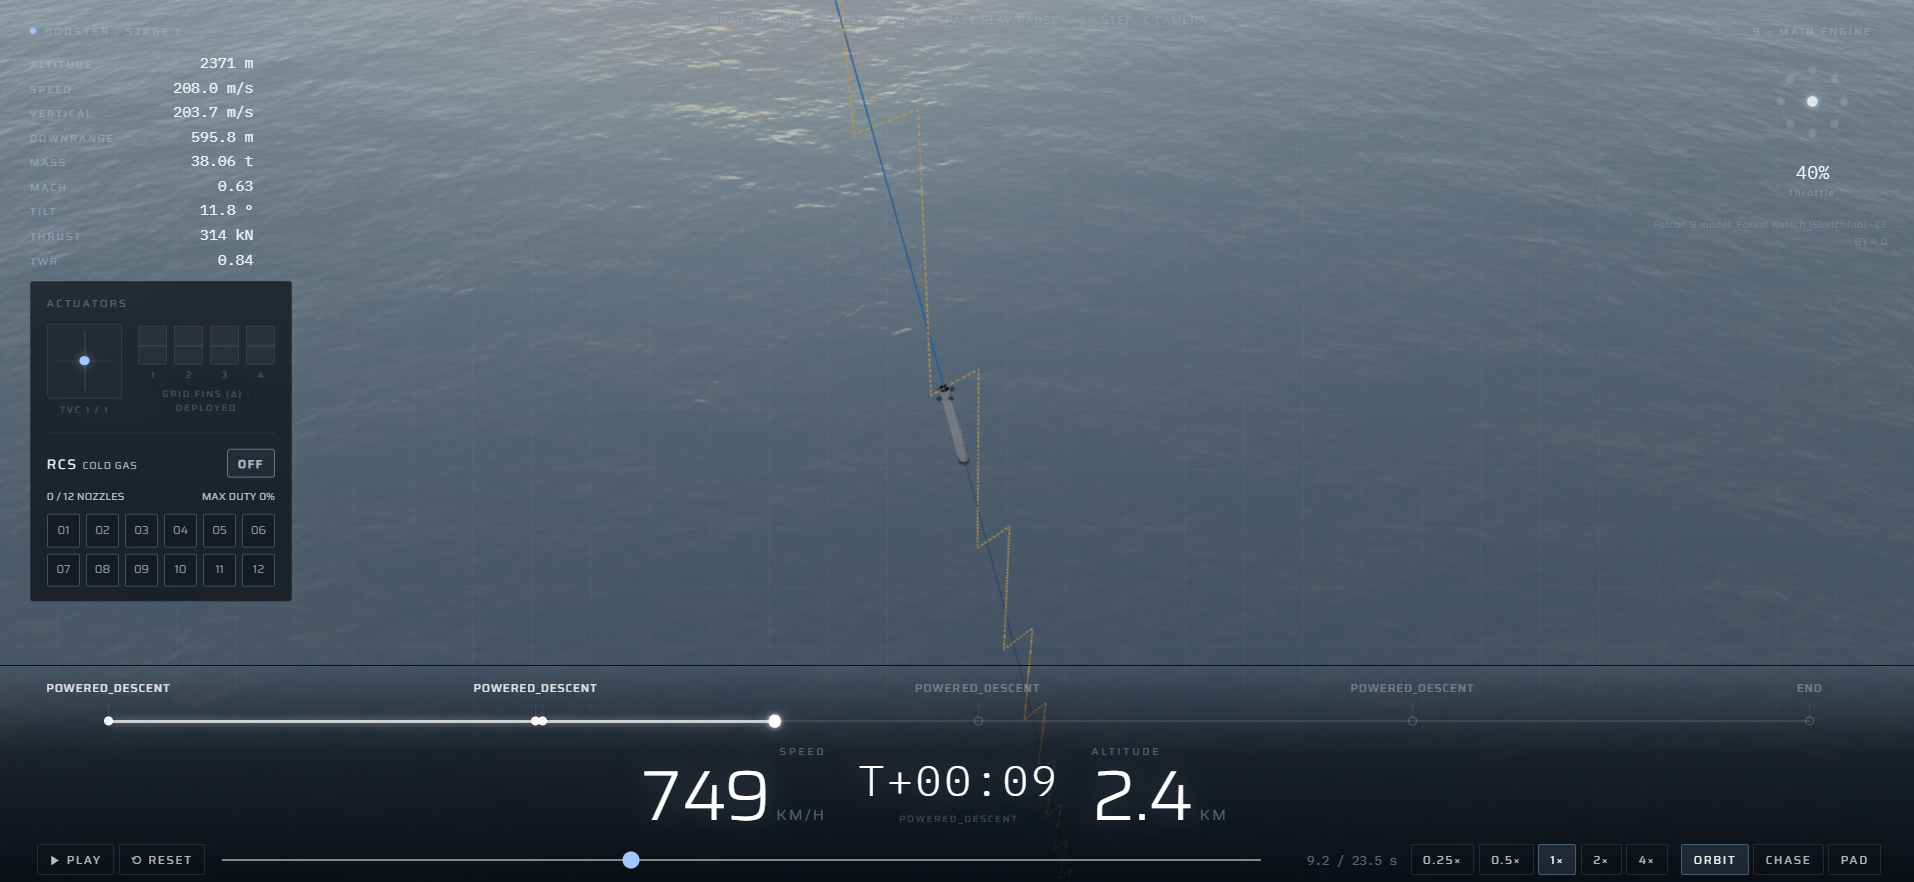
\includegraphics[width=\textwidth]{images/simulator_powered_descent.png}
\par\smallskip{\small (b) Powered descent}\par
\caption{Replay views of unpowered and powered descent. The engine-status display distinguishes the engine-off atmospheric segment from center-engine braking, while the three-dimensional view shows vehicle orientation and grid-fin deployment. Vehicle model: Forest Katsch (Sketchfab, CC BY 4.0).}
\label{fig:replay-descent}
\end{figure}
\end{document}
